% Options for packages loaded elsewhere
\PassOptionsToPackage{unicode}{hyperref}
\PassOptionsToPackage{hyphens}{url}
%
\documentclass[
]{book}
\usepackage{amsmath,amssymb}
\usepackage{iftex}
\ifPDFTeX
  \usepackage[T1]{fontenc}
  \usepackage[utf8]{inputenc}
  \usepackage{textcomp} % provide euro and other symbols
\else % if luatex or xetex
  \usepackage{unicode-math} % this also loads fontspec
  \defaultfontfeatures{Scale=MatchLowercase}
  \defaultfontfeatures[\rmfamily]{Ligatures=TeX,Scale=1}
\fi
\usepackage{lmodern}
\ifPDFTeX\else
  % xetex/luatex font selection
\fi
% Use upquote if available, for straight quotes in verbatim environments
\IfFileExists{upquote.sty}{\usepackage{upquote}}{}
\IfFileExists{microtype.sty}{% use microtype if available
  \usepackage[]{microtype}
  \UseMicrotypeSet[protrusion]{basicmath} % disable protrusion for tt fonts
}{}
\makeatletter
\@ifundefined{KOMAClassName}{% if non-KOMA class
  \IfFileExists{parskip.sty}{%
    \usepackage{parskip}
  }{% else
    \setlength{\parindent}{0pt}
    \setlength{\parskip}{6pt plus 2pt minus 1pt}}
}{% if KOMA class
  \KOMAoptions{parskip=half}}
\makeatother
\usepackage{xcolor}
\usepackage{color}
\usepackage{fancyvrb}
\newcommand{\VerbBar}{|}
\newcommand{\VERB}{\Verb[commandchars=\\\{\}]}
\DefineVerbatimEnvironment{Highlighting}{Verbatim}{commandchars=\\\{\}}
% Add ',fontsize=\small' for more characters per line
\usepackage{framed}
\definecolor{shadecolor}{RGB}{248,248,248}
\newenvironment{Shaded}{\begin{snugshade}}{\end{snugshade}}
\newcommand{\AlertTok}[1]{\textcolor[rgb]{0.94,0.16,0.16}{#1}}
\newcommand{\AnnotationTok}[1]{\textcolor[rgb]{0.56,0.35,0.01}{\textbf{\textit{#1}}}}
\newcommand{\AttributeTok}[1]{\textcolor[rgb]{0.13,0.29,0.53}{#1}}
\newcommand{\BaseNTok}[1]{\textcolor[rgb]{0.00,0.00,0.81}{#1}}
\newcommand{\BuiltInTok}[1]{#1}
\newcommand{\CharTok}[1]{\textcolor[rgb]{0.31,0.60,0.02}{#1}}
\newcommand{\CommentTok}[1]{\textcolor[rgb]{0.56,0.35,0.01}{\textit{#1}}}
\newcommand{\CommentVarTok}[1]{\textcolor[rgb]{0.56,0.35,0.01}{\textbf{\textit{#1}}}}
\newcommand{\ConstantTok}[1]{\textcolor[rgb]{0.56,0.35,0.01}{#1}}
\newcommand{\ControlFlowTok}[1]{\textcolor[rgb]{0.13,0.29,0.53}{\textbf{#1}}}
\newcommand{\DataTypeTok}[1]{\textcolor[rgb]{0.13,0.29,0.53}{#1}}
\newcommand{\DecValTok}[1]{\textcolor[rgb]{0.00,0.00,0.81}{#1}}
\newcommand{\DocumentationTok}[1]{\textcolor[rgb]{0.56,0.35,0.01}{\textbf{\textit{#1}}}}
\newcommand{\ErrorTok}[1]{\textcolor[rgb]{0.64,0.00,0.00}{\textbf{#1}}}
\newcommand{\ExtensionTok}[1]{#1}
\newcommand{\FloatTok}[1]{\textcolor[rgb]{0.00,0.00,0.81}{#1}}
\newcommand{\FunctionTok}[1]{\textcolor[rgb]{0.13,0.29,0.53}{\textbf{#1}}}
\newcommand{\ImportTok}[1]{#1}
\newcommand{\InformationTok}[1]{\textcolor[rgb]{0.56,0.35,0.01}{\textbf{\textit{#1}}}}
\newcommand{\KeywordTok}[1]{\textcolor[rgb]{0.13,0.29,0.53}{\textbf{#1}}}
\newcommand{\NormalTok}[1]{#1}
\newcommand{\OperatorTok}[1]{\textcolor[rgb]{0.81,0.36,0.00}{\textbf{#1}}}
\newcommand{\OtherTok}[1]{\textcolor[rgb]{0.56,0.35,0.01}{#1}}
\newcommand{\PreprocessorTok}[1]{\textcolor[rgb]{0.56,0.35,0.01}{\textit{#1}}}
\newcommand{\RegionMarkerTok}[1]{#1}
\newcommand{\SpecialCharTok}[1]{\textcolor[rgb]{0.81,0.36,0.00}{\textbf{#1}}}
\newcommand{\SpecialStringTok}[1]{\textcolor[rgb]{0.31,0.60,0.02}{#1}}
\newcommand{\StringTok}[1]{\textcolor[rgb]{0.31,0.60,0.02}{#1}}
\newcommand{\VariableTok}[1]{\textcolor[rgb]{0.00,0.00,0.00}{#1}}
\newcommand{\VerbatimStringTok}[1]{\textcolor[rgb]{0.31,0.60,0.02}{#1}}
\newcommand{\WarningTok}[1]{\textcolor[rgb]{0.56,0.35,0.01}{\textbf{\textit{#1}}}}
\usepackage{longtable,booktabs,array}
\usepackage{calc} % for calculating minipage widths
% Correct order of tables after \paragraph or \subparagraph
\usepackage{etoolbox}
\makeatletter
\patchcmd\longtable{\par}{\if@noskipsec\mbox{}\fi\par}{}{}
\makeatother
% Allow footnotes in longtable head/foot
\IfFileExists{footnotehyper.sty}{\usepackage{footnotehyper}}{\usepackage{footnote}}
\makesavenoteenv{longtable}
\usepackage{graphicx}
\makeatletter
\def\maxwidth{\ifdim\Gin@nat@width>\linewidth\linewidth\else\Gin@nat@width\fi}
\def\maxheight{\ifdim\Gin@nat@height>\textheight\textheight\else\Gin@nat@height\fi}
\makeatother
% Scale images if necessary, so that they will not overflow the page
% margins by default, and it is still possible to overwrite the defaults
% using explicit options in \includegraphics[width, height, ...]{}
\setkeys{Gin}{width=\maxwidth,height=\maxheight,keepaspectratio}
% Set default figure placement to htbp
\makeatletter
\def\fps@figure{htbp}
\makeatother
\setlength{\emergencystretch}{3em} % prevent overfull lines
\providecommand{\tightlist}{%
  \setlength{\itemsep}{0pt}\setlength{\parskip}{0pt}}
\setcounter{secnumdepth}{5}
\providecommand{\arrowvert}{}
\usepackage{booktabs}
\usepackage{fancyhdr}
\usepackage{geometry}
\usepackage{titlesec}
\usepackage{etoolbox}
\usepackage{mathptmx}
\geometry{
  top=1in, 
  bottom=1in, 
  left=1in, 
  right=1in, 
  headheight=17pt, 
  includehead, 
  includefoot  
}
\pagestyle{fancy}
\fancyhf{} 
\fancyhead[R]{\thepage} 
\renewcommand{\headrulewidth}{0pt} 
\fancypagestyle{plain}{
  \fancyhf{}
  \fancyhead[R]{\thepage}
  \renewcommand{\headrulewidth}{0pt}
}

\makeatletter
\patchcmd{\chapter}{\if@openright\cleardoublepage\else\clearpage\fi}{\clearpage}{}{}
\makeatother


\titleformat{\section}
  {\normalfont\Large\bfseries\itshape}{\thesection}{1em}{}
\titleformat{\subsection}
  {\normalfont\large\itshape\bfseries}{\thesubsection}{1em}{}
\ifLuaTeX
  \usepackage{selnolig}  % disable illegal ligatures
\fi
\usepackage[]{natbib}
\bibliographystyle{plainnat}
\IfFileExists{bookmark.sty}{\usepackage{bookmark}}{\usepackage{hyperref}}
\IfFileExists{xurl.sty}{\usepackage{xurl}}{} % add URL line breaks if available
\urlstyle{same}
\hypersetup{
  pdftitle={Boston Celtics's Social Media Strategy Analytics Report},
  pdfauthor={Junqi Fu, Zhe Zhou, Zhenghao He, Yucan Zhang, Cassidy Leake},
  hidelinks,
  pdfcreator={LaTeX via pandoc}}

\title{Boston Celtics's Social Media Strategy Analytics Report}
\author{Junqi Fu, Zhe Zhou, Zhenghao He, Yucan Zhang, Cassidy Leake}
\date{2023-12-13}

\begin{document}
\maketitle

{
\setcounter{tocdepth}{1}
\tableofcontents
}
\hypertarget{executive-summary}{%
\chapter{Executive Summary}\label{executive-summary}}

This report presents a comprehensive analysis and strategic plan for enhancing fan engagement of the Boston Celtics on online community. Utilizing advanced data analytics methods and tools such as automated text anallytics, network modeling, and social listening, we have scrutinized a year's worth of social media data, focusing on two major social media platforms: Twitter/X and TikTok. Our finings reveal distinct patterns in Celtics' fan online engagement, underscoring the potential of TikTok as a highly interactive community and Twitter/X as a hub for online engagements.

Based on our data analysis, we propose the ``\#BleedGreen'' campaign for TikTok and a pre-playoff campaign for Twitter/X. Leverage insights from social data, we aim to utilize these campaign to foster a stronger connection between the Celtics and our fan base. On TikTok, we aim to capitalize on the popularity of Celtics-related sportswear and appearl, encouraging fans to actively connect their interested contents and their Celtics pride.For Twitter/X, we focus on enhancing conversations around the franchise, using advanced computational approaches to identify and stimulate metrics that can drive fan engagement.

Our strategic approach balances the rich history and local community ties of the franchise with the dynamic and evolving nature of social media engagement, positioning the Boston Celtics for continued success both on and off the court.

\hypertarget{statement-of-purpose-and-objectives}{%
\chapter{Statement of Purpose and Objectives}\label{statement-of-purpose-and-objectives}}

The goal of this social media strategy is to enhance positive interactions between official Celtics tweets and fans.

To achieve this goal, we will utilize insights from social text data and user engagement data across various social media platforms, which will help us craft customized strategies and campaigns tailored for popular social media platforms. Our objectives are twofold: 1) significantly boost user engagement in online discussions, and 2) greatly increase positive sentiment in Twitter conversations about the Boston Celtics, aiming for an overall 24\% positivity rate in these discussions.

\hypertarget{celtics-its-background}{%
\chapter{Celtics \& Its Background}\label{celtics-its-background}}

\hypertarget{boston-celtics}{%
\section{Boston Celtics}\label{boston-celtics}}

The Boston Celtics, one of the oldest and domiannt NBA franchises, boasts a rich history and has significantly influenced the development of both the National Basketball Association and basketball as a prominent Olympic sport genre.

Since its founding in Boston in 1946 \citep{britannica2023bostonceltics}, the evolution of its core fan culture has been significantly shaped and driven by the sports fan community in Boston. This fan base gradually extended to encompass the greater New England area, with Boston as its focal point (see below table 3.1).

\begin{Shaded}
\begin{Highlighting}[]
\FunctionTok{ggplot}\NormalTok{(long\_data, }\FunctionTok{aes}\NormalTok{(}\AttributeTok{x=}\FunctionTok{reorder}\NormalTok{(Region, Score), }\AttributeTok{y=}\NormalTok{Score, }\AttributeTok{fill=}\NormalTok{Score\_Type)) }\SpecialCharTok{+} 
  \FunctionTok{geom\_bar}\NormalTok{(}\AttributeTok{stat=}\StringTok{"identity"}\NormalTok{) }\SpecialCharTok{+}
  \FunctionTok{coord\_flip}\NormalTok{() }\SpecialCharTok{+}
  \FunctionTok{theme\_minimal}\NormalTok{() }\SpecialCharTok{+}
  \FunctionTok{labs}\NormalTok{(}\AttributeTok{title=}\StringTok{"Table 3.1: Google Trends: Boston Celtics\textquotesingle{}s Online Mention By Region"}\NormalTok{, }\AttributeTok{x=}\StringTok{"Region"}\NormalTok{, }\AttributeTok{y=}\StringTok{"Mention"}\NormalTok{)}
\end{Highlighting}
\end{Shaded}

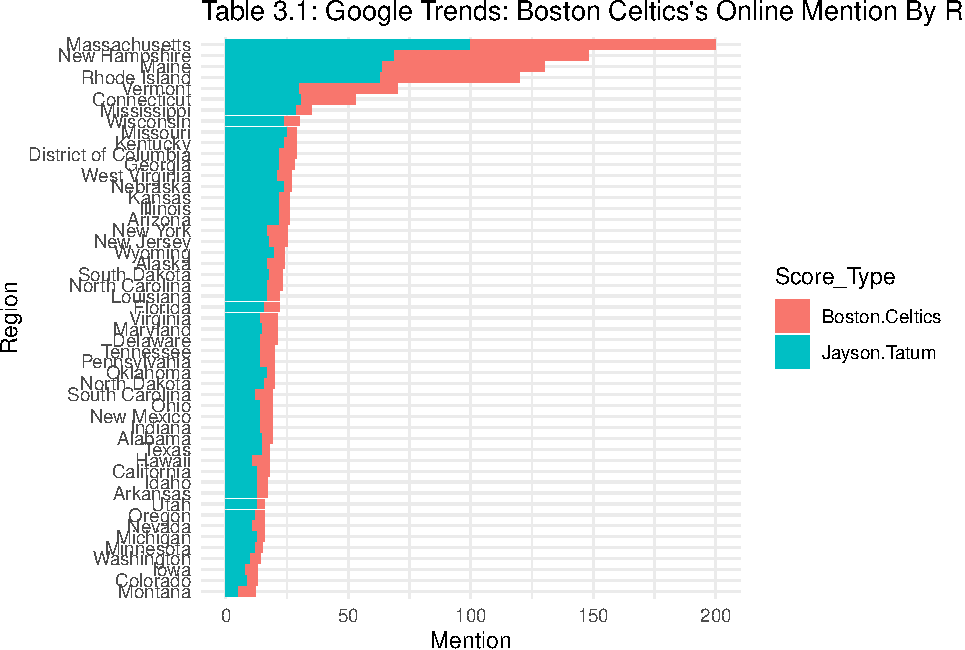
\includegraphics{_main_files/figure-latex/unnamed-chunk-2-1.pdf}

\hypertarget{celticss-target-audiences}{%
\section{Celtics's Target Audiences}\label{celticss-target-audiences}}

As partially reflected in table 3.1, the primary target fans and audience for the Boston Celtics are long-time basketball enthusiasts who identify themselves as sports fans in the city of Boston or the broader New England area. These fans particularly appreciate the team's historical success in the city. This preference aligns with the old tradition of the local Boston community, contributing to a strong Boston's local sports fan culture \citep{olguin2022magnetismceltics}.

The Celtics' fan culture and its connection to Boston's sports culture were significantly bolstered by the franchise's history of winning 17 championship titles. This achievement historically ties the Celtics with another of the NBA's greatest franchises, the LA Lakers, as they share the record for the most championships in league history. Additionally, the rivalry between these two teams has been a defining aspect of the NBA, particularly during iconic eras such as the Bill Russell (Celtics) and Jerry West (Lakers) era in the 1960s, the Larry Bird (Celtics) and Magic Johnson (Lakers) era in the 1980s, and the late 2000s rivalry between the Celtics' Big Three and Kobe Bryant of the Lakers. These historic matchups are officially cited as highlights of NBA history. Such a storied rivalry with the LA Lakers adds a unique dimension to the Celtics' brand narrative, further enriching its sports culture in Boston and the special rivalry tradition between the city of Boston and LA \citep{talkbasket2022celticshistory}.

\hypertarget{la-lakers-primary-competitor}{%
\section{LA Lakers: Primary Competitor}\label{la-lakers-primary-competitor}}

However, when compared to Celtics's primary competitor, particularly considering developments over the past 30 years, the LA Lakers have become a franchise with a significantly higher market value and a much larger international and national fan community \citep[e.g.,][]{sam2023nba, skysports2021celticslakers}.

Compared to Boston, the LA Lakers and its owners built the franchise's culture on the historical and rapid development of West Coast pop culture, particularly Hollywood. Enhanced greatly by LA's entertainment industry and Hollywood, the Lakers have not only gained much more exposure but also built a successful star-centered culture. This culture revolves around its star players, including Magic Johnson and Kareem Abdul-Jabbar in the 1980s, Shaquille O'Neal and Kobe Bryant in the last two decades, and LeBron James and Anthony Davis since the 2020s \citep{hbo2023winningtime}.

Furthermore, unlike Boston, which is traditionally regarded as a city centered around white culture, the Lakers appeal to a fan base with a more diverse racial and cultural background nationally and internationally. This contrast was particularly significant in the 1980s when the Celtics' white star, Larry Bird, was seen as the hero of Boston, contrasting with the Lakers' Magic Johnson, who was beloved by the culturally diverse LA fan base \citep{hbo2023winningtime}.

Despite the perception that the Celtics are less competitive in expanding their fan base and attracting new international fans, their consistent connections to the local Boston community have successfully maintained generations of support from Celtics fans and their families in Boston. As shown in Table 1, this steadfast engagement with the local community highlights the Celtics' core strength in increasing fan engagement within its own community.

\hypertarget{data-analytics-plan-and-procedures}{%
\chapter{Data Analytics Plan and Procedures}\label{data-analytics-plan-and-procedures}}

We collected large social data mentioning Celtics mainly primarily through the social listening platform Meltwater. Additionally, we placed particular emphasis on monitoring online discussions on platforms such as Twitter/X, ensuring a comprehensive understanding of the public sentiment and engagement related to the Celtics.

\hypertarget{data-collection-from-meltwater}{%
\section{Data Collection from Meltwater}\label{data-collection-from-meltwater}}

To analyze general audience engagement trends over a year, we utilized Meltwater with a time range filter set from October 18, 2022 (the beginning of NBA 2022-2023 season), to October 17, 2023. Given the franchise's particular focus on fans and supporters in the city of Boston, locations of the collected data are also specified as limited in Boston. This analysis focuses on popular social media platforms, including Twitter, Reddit, TikTok, and Pinterest. The engagement data collected from Meltwater includes various metrics and insights that help us understand how users interact with content related to the Celtics across these platforms. Here's an overview of the engagement data we collected:

\begin{itemize}
\item
  \textbf{Mentions trend by source}
\item
  \textbf{Engagement trend by source}
\item
  \textbf{Sentiment distribution by source}
\item
  \textbf{Top words and hashtags}
\end{itemize}

\hypertarget{twitterx-data-collection-analytics}{%
\section{Twitter/X Data Collection \& Analytics}\label{twitterx-data-collection-analytics}}

\hypertarget{boolean-logic-search-query-for-twitterx-data-collection}{%
\subsection{Boolean Logic Search Query for Twitter/X Data Collection}\label{boolean-logic-search-query-for-twitterx-data-collection}}

``(''boston celtics`` OR ''\#celtics`` OR ''@celtics`` OR ''\#bleedgreen`` OR ''\#celticsnation`` OR
''\#celticsgameday`` OR ``\#celticswin'' OR ``jayson tatum'' OR ``jaylen brown'' OR ``al horford'' OR ``celtics vs'' OR ``celtics trade'' OR ``celtics draft'' OR ``celtics roster'' OR ``celtics injury'' OR ``celtics score'' OR ``celtics highlights'' OR ``celtics playoffs'' OR ``celtics finals'' OR ``celtics championship'' OR ``celtics rumors'' OR ``celtics signings'' OR ``celtics defense'' OR ``celtics offense'' OR ``\#greenrunsdeep'' OR ``\#banner18'') NOT (``green'' OR ``basketball'' OR ``nba'')''

Utilizing a boolean logic search query, a sample of 20,000 tweets was collected from Meltwater, spanning from October 18, 2022, to October 17, 2023, sent/replied in Boston. The data analysis procedure concentrated on using tweets as the unit of analysis. To achieve the objective of boosting user engagement and increasing overall positive conversations in the online community, the analysis of tweet data primarily focused on two major metrics: tweet reach (engagement) and sentiment.

Additionally, by creating a new variable labeled ``topic'' for each tweet, the aim is to specialize our focus on promoting user engagement in conversations specifically centered around the franchise, rather than solely focusing on all-star players or game-focused discussions. This approach allows for a more targeted strategy in enhancing the engagement and sentiment within the Celtics' online community.

\hypertarget{insights-from-data-analytics}{%
\chapter{Insights From Data Analytics}\label{insights-from-data-analytics}}

\hypertarget{insights-from-meltwaters-user-engagement-data}{%
\section{Insights from Meltwater's User Engagement Data}\label{insights-from-meltwaters-user-engagement-data}}

\hypertarget{mentions-distribution-by-sources}{%
\subsection{Mentions Distribution by Sources}\label{mentions-distribution-by-sources}}

From October 2022 to October 2023, Twitter/X and Reddit have been identified as the most popular channels for online discussions about the Celtics, with their conversation volumes reaching over millions (see figure 5.1). Additionally, throughout this time range, there were several noticeable peaks in the overall conversation volume. These peaks likely correspond to highlight events involving the franchise, such as the game against the Brooklyn Nets, led by Kevin Durant on December 4, and the Eastern Conference Finals against the Miami Heat starting in mid-May 2023. These key events seem to have significantly driven online posts among the fan base.

\begin{figure}
\centering
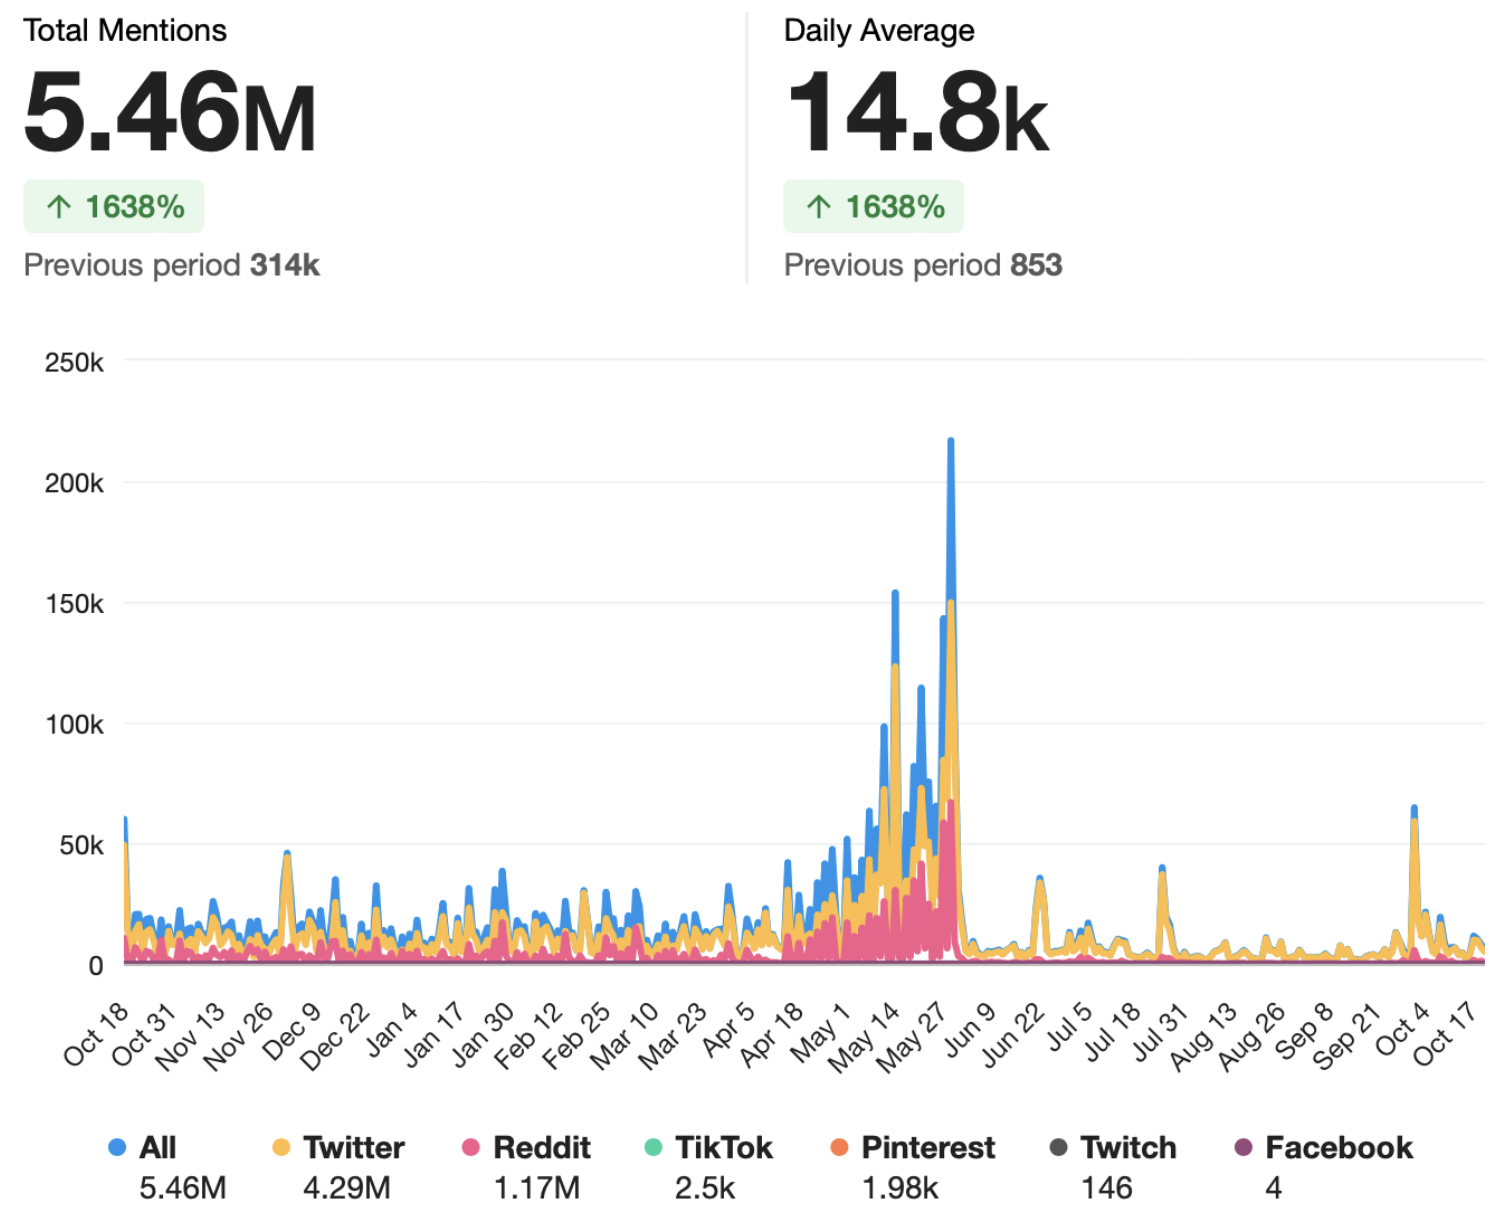
\includegraphics{1.png}
\caption{Mentions trend by source}
\end{figure}

\hypertarget{engagement-distribution-by-sources}{%
\subsection{Engagement Distribution by Sources}\label{engagement-distribution-by-sources}}

However, The total engagement metrics, which include likes, shares, and comments, reveal an interesting trend: although there are significantly fewer mentions of the Celtics on TikTok compared to Twitter/X and Reddit, the content related to the Celtics on TikTok is highly interactive and likely includes viral video content. Specifically, on TikTok, the ratio of engagement to mentions is a crazily staggering 5200 (i.e., 13 million engagements for 0.025 million mentions), indicating a very high level of user interaction per post. In contrast, on Twitter/X and Reddit, this metric is much lower, with ratios of 7.25 and 7.74 (see figure 5.1 and 5.2). This disparity suggests that while Twitter and Reddit have higher volumes of conversation, TikTok's content has a significantly greater capacity for engagement per mention.

\begin{figure}
\centering
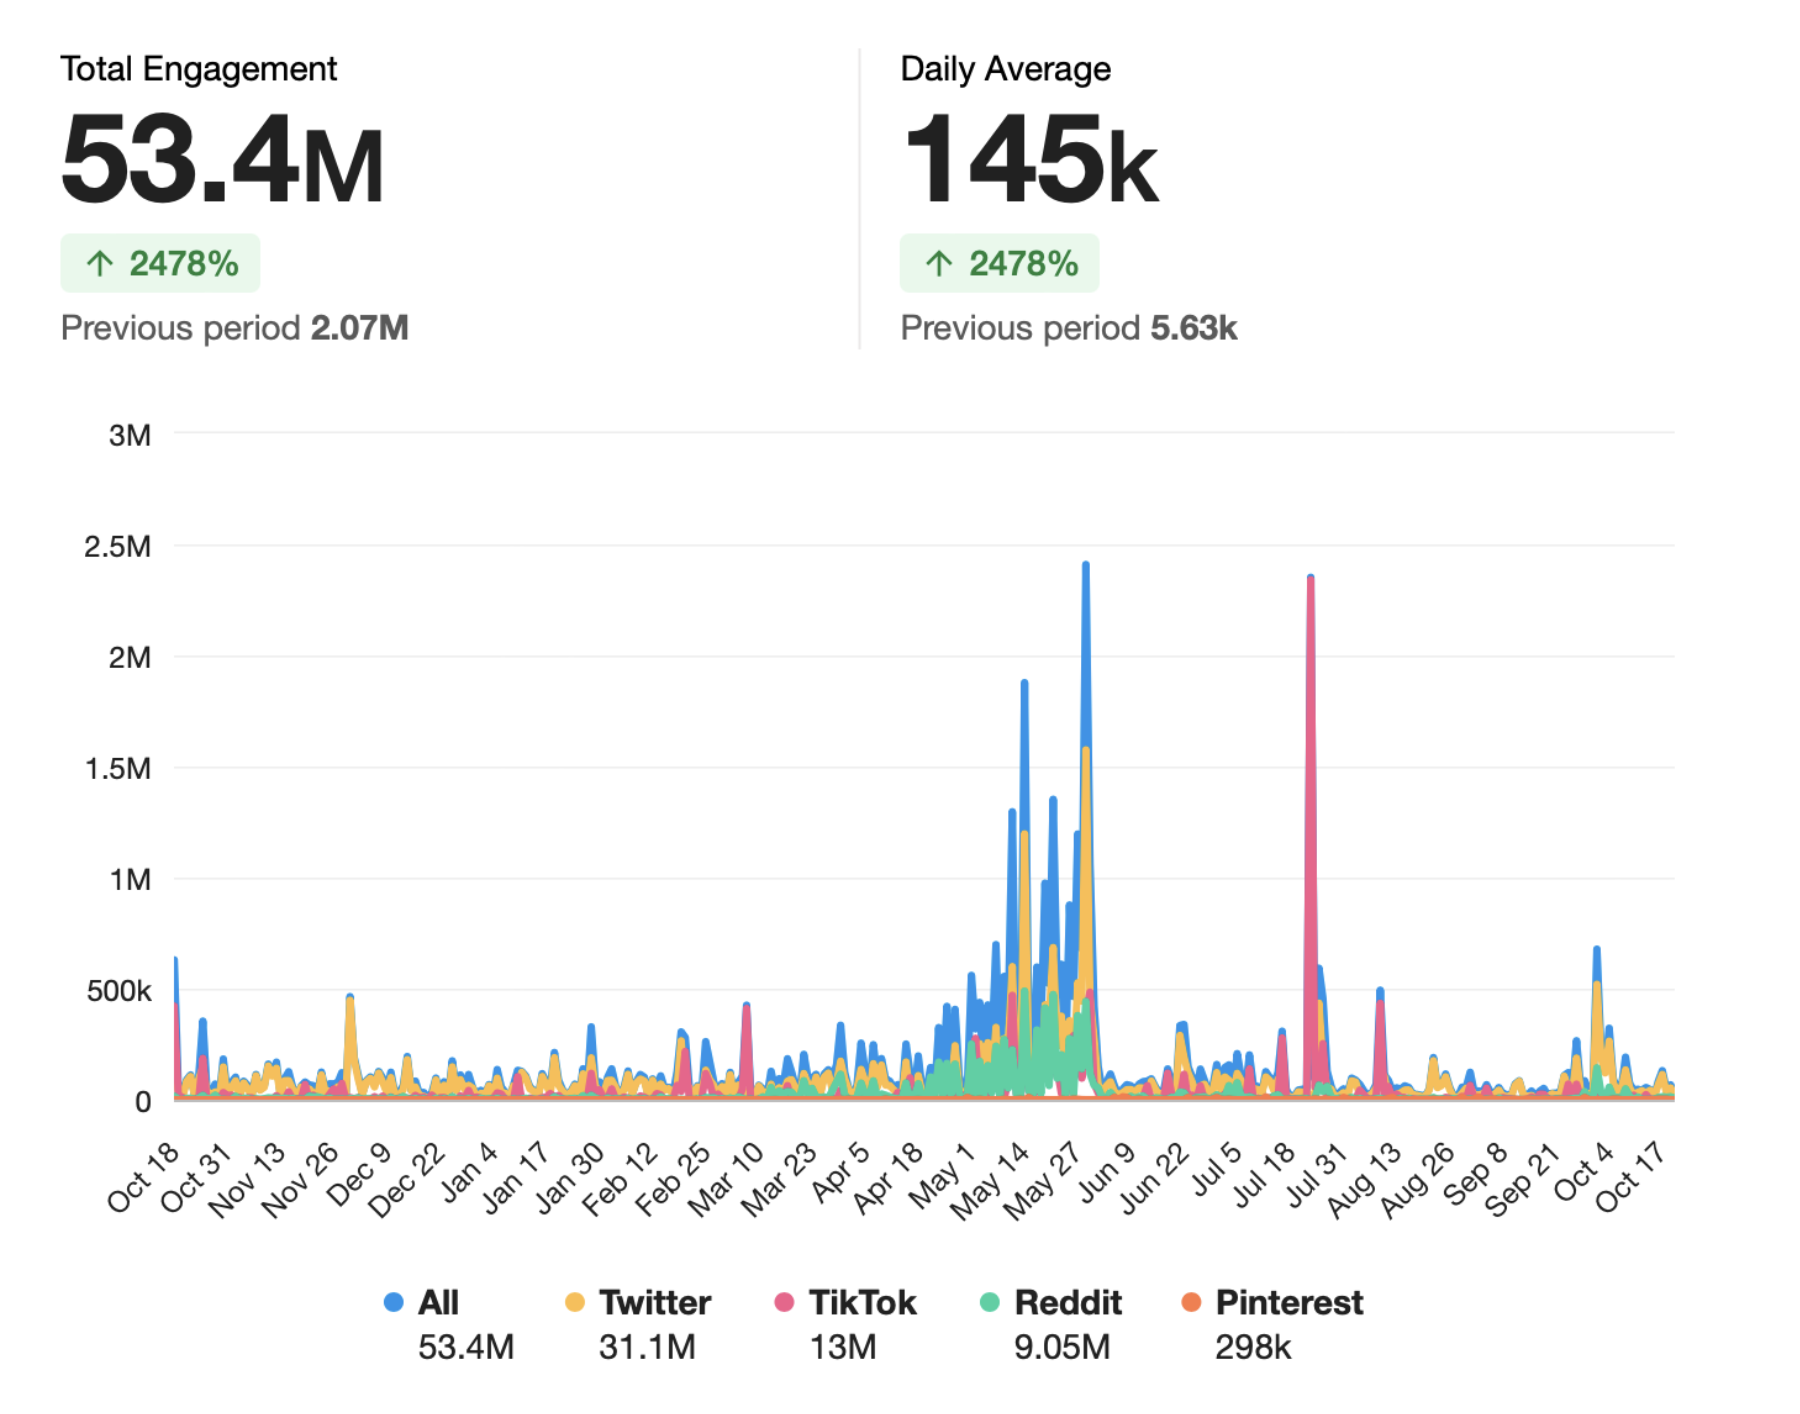
\includegraphics{2.png}
\caption{Engagement trend by source}
\end{figure}

\hypertarget{sentiment-by-sources}{%
\subsection{Sentiment by Sources}\label{sentiment-by-sources}}

Additionally, compared to toher platforms, conversations about Celtics on TikTok is much more positive, which could indicate that the generated contents by fans there is both entertaining and favorable towards the Celtics (see figure 5.3).

\begin{figure}
\centering
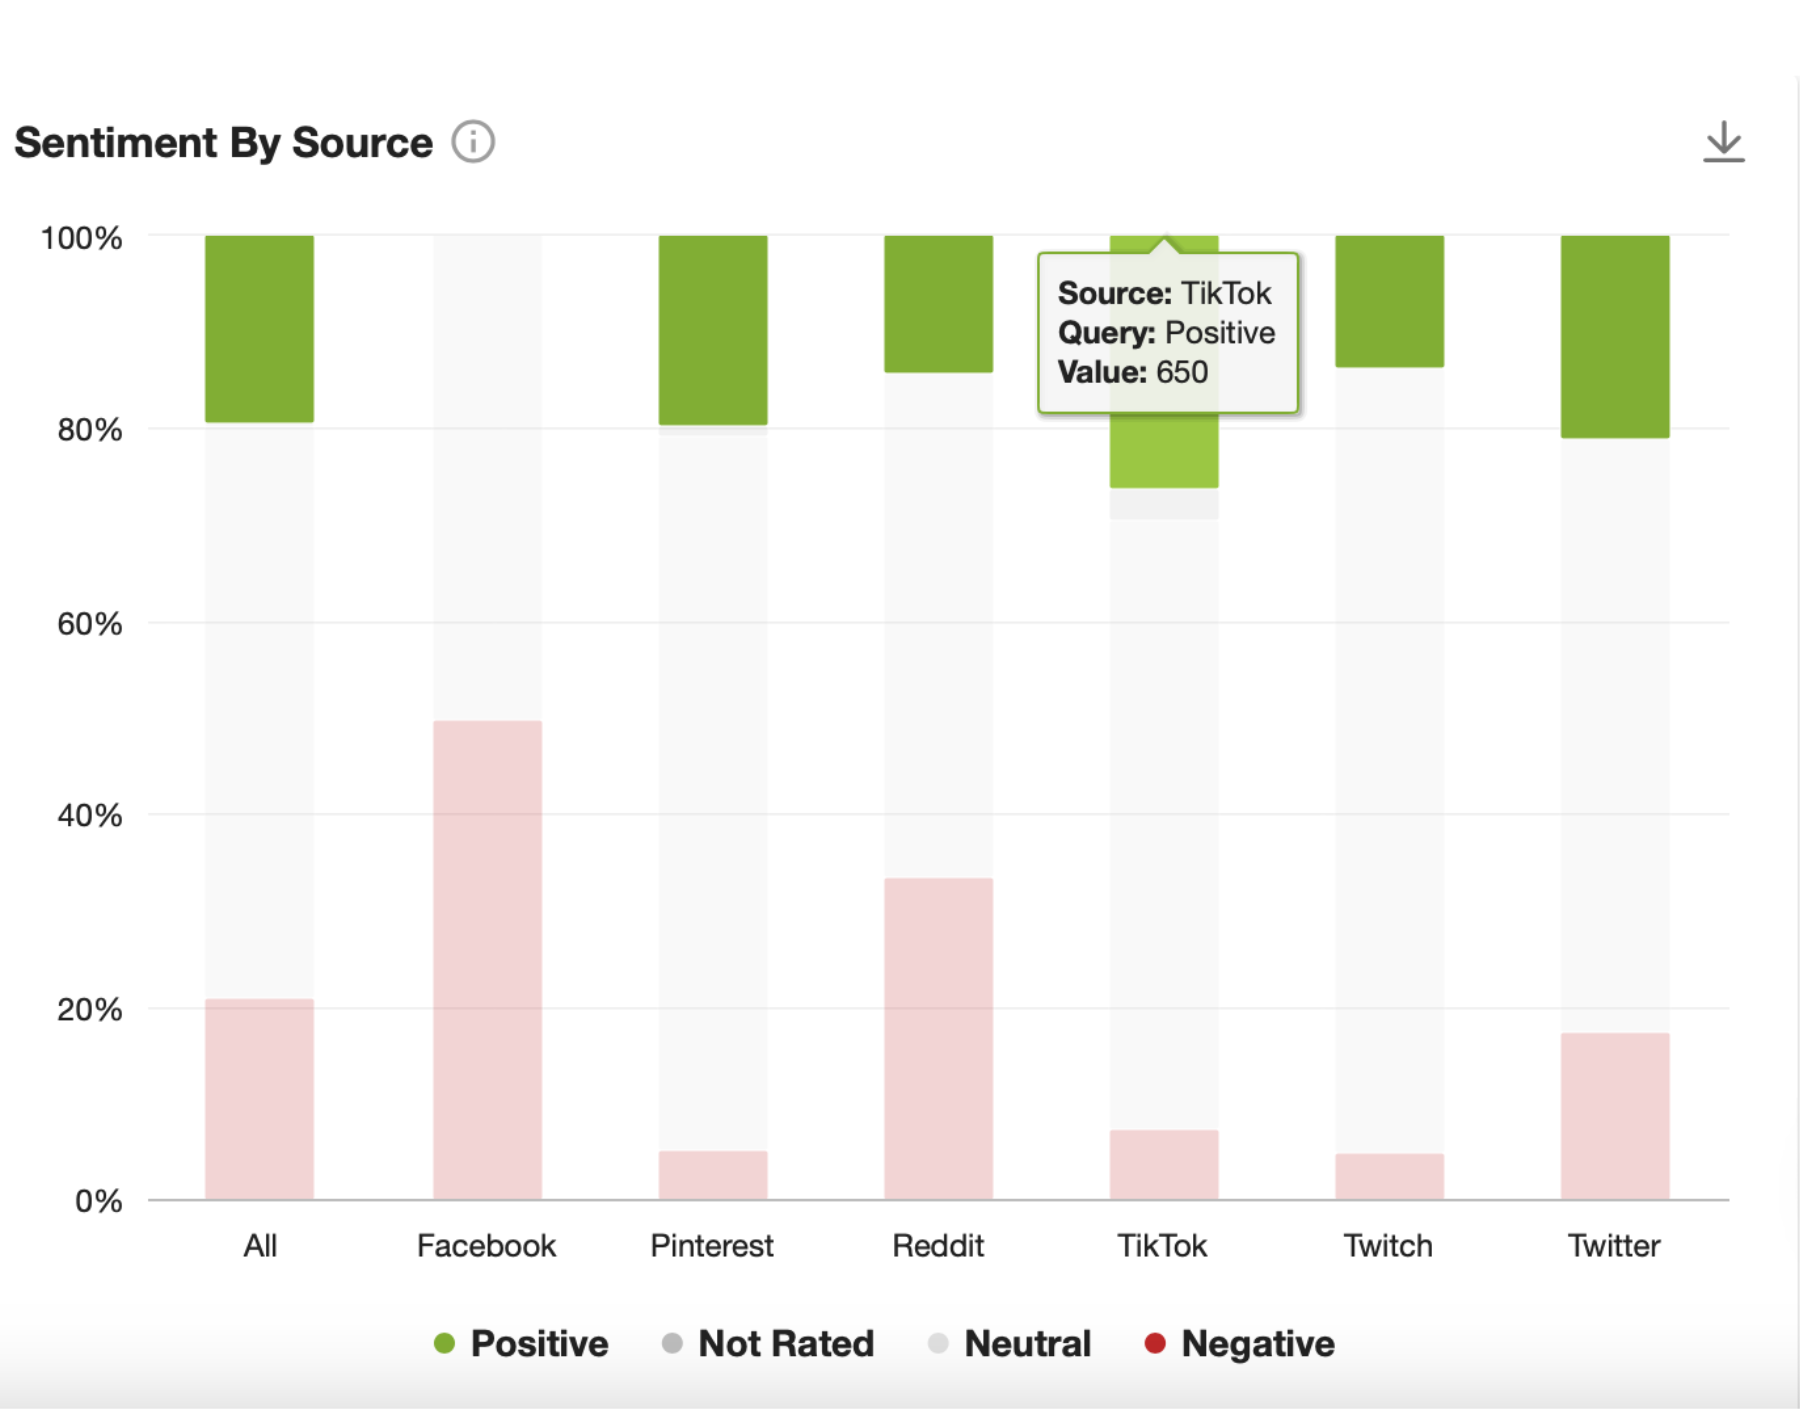
\includegraphics{3.png}
\caption{Sentiment by source}
\end{figure}

\hypertarget{a-customized-campaign-to-enahnce-engagement-on-tiktok}{%
\subsection{A Customized Campaign to Enahnce Engagement on TikTok}\label{a-customized-campaign-to-enahnce-engagement-on-tiktok}}

Given these insights, while Twitter/X is recognized as the central hub for Celtics-related conversations and interactions, TikTok emerges as a platform with high potential for building a favorable fan community. Its ability to enhance positive online discussions about the franchise and unite fans is particularly notable due to its high engagement ratio. The interactive and often viral nature of content on TikTok can be leveraged to foster a more engaged and enthusiastic fan community, contributing significantly to the overall positive sentiment and visibility of the Celtics brand in the digital space.

\hypertarget{insights-from-twitterx-data}{%
\section{Insights from Twitter/X Data}\label{insights-from-twitterx-data}}

\hypertarget{reach-distribution-by-topics}{%
\subsection{Reach Distribution by Topics}\label{reach-distribution-by-topics}}

\begin{Shaded}
\begin{Highlighting}[]
\NormalTok{lda.model }\OtherTok{\textless{}{-}} \FunctionTok{LDA}\NormalTok{(myDTM, }\DecValTok{10}\NormalTok{, }\AttributeTok{method=}\StringTok{\textquotesingle{}Gibbs\textquotesingle{}}\NormalTok{, }\AttributeTok{control=}\FunctionTok{list}\NormalTok{(}\AttributeTok{seed=}\DecValTok{2022}\NormalTok{))}

\NormalTok{topic\_matrix }\OtherTok{\textless{}{-}} \FunctionTok{terms}\NormalTok{(lda.model,}\DecValTok{10}\NormalTok{) }
\NormalTok{topic\_matrix}
\end{Highlighting}
\end{Shaded}

\begin{verbatim}
##       Topic 1    Topic 2   Topic 3   Topic 4              Topic 5     
##  [1,] "time"     "tatum"   "brown"   "game"               "win"       
##  [2,] "will"     "jayson"  "jaylen"  "tonight"            "get"       
##  [3,] "thank"    "mvp"     "trade"   "bleedgreen"         "bleedgreen"
##  [4,] "mazzulla" "embiid"  "via"     "night"              "now"       
##  [5,] "joe"      "kevin"   "per"     "heat"               "let"       
##  [6,] "coach"    "top"     "star"    "unfinishedbusiness" "don"       
##  [7,] "tell"     "giannis" "says"    "finals"             "big"       
##  [8,] "efforts"  "jimmy"   "without" "series"             "new"       
##  [9,] "sources"  "butler"  "lillard" "business"           "need"      
## [10,] "years"    "joel"    "jordan"  "miami"              "today"     
##       Topic 6   Topic 7  Topic 8  Topic 9    Topic 10
##  [1,] "can"     "just"   "team"   "back"     "season"
##  [2,] "like"    "got"    "year"   "horford"  "points"
##  [3,] "good"    "love"   "one"    "smart"    "pts"   
##  [4,] "play"    "fans"   "best"   "williams" "games" 
##  [5,] "going"   "see"    "player" "marcus"   "first" 
##  [6,] "said"    "know"   "two"    "left"     "last"  
##  [7,] "great"   "even"   "still"  "white"    "reb"   
##  [8,] "think"   "live"   "league" "right"    "ast"   
##  [9,] "better"  "fan"    "next"   "brogdon"  "point" 
## [10,] "defense" "people" "way"    "derrick"  "career"
\end{verbatim}

\begin{verbatim}
##   document       topic
## 1        1           7
## 2        2           6
## 3        3 1, 5, 7, 10
## 4        4           6
## 5        5       1, 10
## 6        6           6
\end{verbatim}

\hypertarget{topic-categories}{%
\subsubsection{Topic Categories:}\label{topic-categories}}

Utilizing the Latent Dirichlet Allocation (LDA) unsupervised topic modeling method \citep{chen2011latentdirichlet}, an analysis of the Celtics-related conversations yielded 10 salient topics (see above results and below summary). Among these topics, our special focus is directed towards conversations centered on fan engagement topics (i.e., topic category 4).

This topic category likely encapsulates discussions that are directly relevant to increasing user engagement and fostering a strong fan community. By focusing on this category, efforts can be more effectively channeled towards strategies that resonate with the fans' interests and preferences, thereby amplifying engagement and participation in online discussions about the franchise.

\textbf{Category 1: Star Player}

\begin{itemize}
\item
  Topic 2: Centers around Jayson Tatum and related MVP title discussion
\item
  Topic 3: Jaylen Brown and potential trade rumors
\end{itemize}

\textbf{Category 2: Game}

\begin{itemize}
\item
  Topic 1: Timing of games/events
\item
  Topic 6: Strategies/opinions on games
\end{itemize}

\textbf{Category 3: Franchise Management}

\begin{itemize}
\item
  Topic 8: Team Management
\item
  Topic 9: Other players
\end{itemize}

\textbf{Category 4: Fan Engagement}

\begin{itemize}
\item
  Topic 4: Celtics slogan
\item
  Topic 5: Appeal for wining and achievements
\item
  Topic 7: Fans community
\item
  Topic 10: Season statistics \& Career achievements
\end{itemize}

\hypertarget{topic-tweets-daily-reach}{%
\subsubsection{Topic \& Tweets Daily Reach}\label{topic-tweets-daily-reach}}

A visualized plot was created to analyze the daily reach of tweets under each topic category over the course of a year (see figure 5.4). This visualization helps in understanding how the reach of different conversation topics fluctuates over time. Additionally, to understand whether conversations related to fan engagement potentially achieve a higher level of daily reach, a one-sided two-sample t-test was employed.

However, both from visual inspection (the ``eye-ball'' method) and the statistical results, it appears that conversations centered around fan engagement do not demonstrate a significantly different level of daily reach (\mu = 24458.26) or a distinct pattern in the distribution of their reach.

\begin{Shaded}
\begin{Highlighting}[]
\NormalTok{tt}\OtherTok{\textless{}{-}}\FunctionTok{ggplot}\NormalTok{(data\_1,}\FunctionTok{aes}\NormalTok{(}\AttributeTok{x=}\NormalTok{Day,}\AttributeTok{y=}\NormalTok{Daily\_Reach,}\AttributeTok{group=}\FunctionTok{as.factor}\NormalTok{(topic),}\AttributeTok{color=}\FunctionTok{as.factor}\NormalTok{(topic))) }\SpecialCharTok{+}
  \FunctionTok{geom\_line}\NormalTok{() }\SpecialCharTok{+} \FunctionTok{geom\_point}\NormalTok{() }\SpecialCharTok{+}
  \FunctionTok{labs}\NormalTok{(}\AttributeTok{title =} \StringTok{"Figure 5.4: Topic Rearch Transition"}\NormalTok{, }\AttributeTok{x =} \StringTok{"Day"}\NormalTok{, }\AttributeTok{y =} \StringTok{"Daily Reach"}\NormalTok{) }\SpecialCharTok{+}
  \FunctionTok{theme\_minimal}\NormalTok{()}
\NormalTok{t }\OtherTok{\textless{}{-}} \FunctionTok{ggplotly}\NormalTok{(tt)}
\NormalTok{t}
\end{Highlighting}
\end{Shaded}

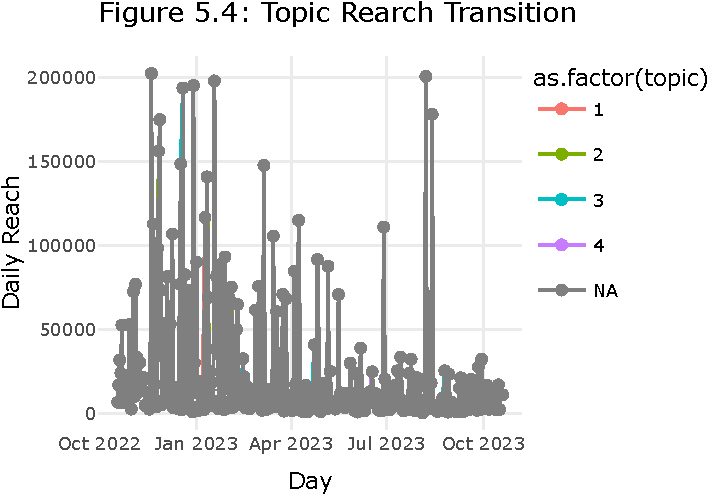
\includegraphics{_main_files/figure-latex/unnamed-chunk-10-1.pdf}

\begin{Shaded}
\begin{Highlighting}[]
\FunctionTok{t.test}\NormalTok{(fan}\SpecialCharTok{$}\NormalTok{Daily\_Reach,other\_topic}\SpecialCharTok{$}\NormalTok{Daily\_Reach,}\AttributeTok{paired=}\ConstantTok{FALSE}\NormalTok{,}\AttributeTok{alternative=}\StringTok{"greater"}\NormalTok{)}
\end{Highlighting}
\end{Shaded}

\begin{verbatim}
## 
##  Welch Two Sample t-test
## 
## data:  fan$Daily_Reach and other_topic$Daily_Reach
## t = 0.60437, df = 11007, p-value = 0.2728
## alternative hypothesis: true difference in means is greater than 0
## 95 percent confidence interval:
##  -647.1339       Inf
## sample estimates:
## mean of x mean of y 
##  24458.26  24082.42
\end{verbatim}

\hypertarget{reach-distribution-by-sentiment}{%
\subsection{Reach Distribution by Sentiment}\label{reach-distribution-by-sentiment}}

Additionally, employing the ``Syuzhet'' package in R, a sentiment analysis was performed on the sample data.

A visualized plot was then created to track the daily reach transitions of tweets categorized by their sentiments (see figure 5.5). On the other hand, to delve deeper into the changes in daily reach among conversations with different sentiments, simple linear regression was utilized.

Reflected in both figure 5.5 and the regression results, there's a overall decreasing trend in the daily reach of tweets with positive sentiments. Specifically, each additional day is associated with a decrease of 144 daily reach, indicating a significant negative trend over time for tweets with positive sentiment. Meanwhile, for tweets with negative sentiment, daily reach also decreases by about 164 with each day.

\begin{Shaded}
\begin{Highlighting}[]
\NormalTok{gg}\OtherTok{\textless{}{-}}\FunctionTok{ggplot}\NormalTok{(data,}\FunctionTok{aes}\NormalTok{(}\AttributeTok{x=}\NormalTok{Day,}\AttributeTok{y=}\NormalTok{Daily\_Reach,}\AttributeTok{group=}\NormalTok{sentiment,}\AttributeTok{color=}\NormalTok{sentiment)) }\SpecialCharTok{+}
  \FunctionTok{geom\_line}\NormalTok{() }\SpecialCharTok{+} \FunctionTok{geom\_point}\NormalTok{() }\SpecialCharTok{+}
  \FunctionTok{labs}\NormalTok{(}\AttributeTok{title =} \StringTok{"Figure 5.5: Sentiment Rearch Transition"}\NormalTok{, }\AttributeTok{x =} \StringTok{"Day"}\NormalTok{, }\AttributeTok{y =} \StringTok{"Daily Reach"}\NormalTok{) }\SpecialCharTok{+}
  \FunctionTok{theme\_minimal}\NormalTok{()}

\NormalTok{p }\OtherTok{\textless{}{-}} \FunctionTok{ggplotly}\NormalTok{(gg)}
\NormalTok{p}
\end{Highlighting}
\end{Shaded}

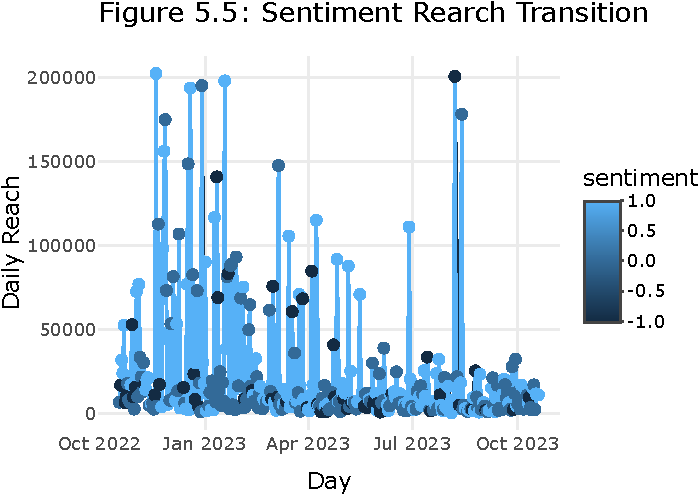
\includegraphics{_main_files/figure-latex/unnamed-chunk-13-1.pdf}

\begin{Shaded}
\begin{Highlighting}[]
\NormalTok{reg\_1}\OtherTok{\textless{}{-}}\FunctionTok{lm}\NormalTok{(Daily\_Reach}\SpecialCharTok{\textasciitilde{}}\NormalTok{Day,positive\_sentiment)}
\NormalTok{reg\_2}\OtherTok{\textless{}{-}}\FunctionTok{lm}\NormalTok{(Daily\_Reach}\SpecialCharTok{\textasciitilde{}}\NormalTok{Day,negative\_sentiment)}
\FunctionTok{stargazer}\NormalTok{(reg\_1,reg\_2,}\AttributeTok{type=}\StringTok{"text"}\NormalTok{,}\AttributeTok{star.cutoffs=}\FunctionTok{c}\NormalTok{(.}\DecValTok{05}\NormalTok{,.}\DecValTok{01}\NormalTok{,.}\DecValTok{001}\NormalTok{))}
\end{Highlighting}
\end{Shaded}

\begin{verbatim}
## 
## =======================================================================
##                                     Dependent variable:                
##                     ---------------------------------------------------
##                                         Daily_Reach                    
##                                (1)                       (2)           
## -----------------------------------------------------------------------
## Day                        -144.021***               -164.246***       
##                              (5.797)                   (8.748)         
##                                                                        
## Constant                2,823,105.000***          3,216,784.000***     
##                           (112,601.000)             (169,943.400)      
##                                                                        
## -----------------------------------------------------------------------
## Observations                  6,020                     2,609          
## R2                            0.093                     0.119          
## Adjusted R2                   0.093                     0.119          
## Residual Std. Error  33,668.440 (df = 6018)    32,533.770 (df = 2607)  
## F Statistic         617.201*** (df = 1; 6018) 352.500*** (df = 1; 2607)
## =======================================================================
## Note:                                     *p<0.05; **p<0.01; ***p<0.001
\end{verbatim}

\begin{Shaded}
\begin{Highlighting}[]
\FunctionTok{plot}\NormalTok{(positive\_sentiment}\SpecialCharTok{$}\NormalTok{Daily\_Reach}\SpecialCharTok{\textasciitilde{}}\NormalTok{positive\_sentiment}\SpecialCharTok{$}\NormalTok{Day)}
\FunctionTok{abline}\NormalTok{(reg\_1)}
\end{Highlighting}
\end{Shaded}

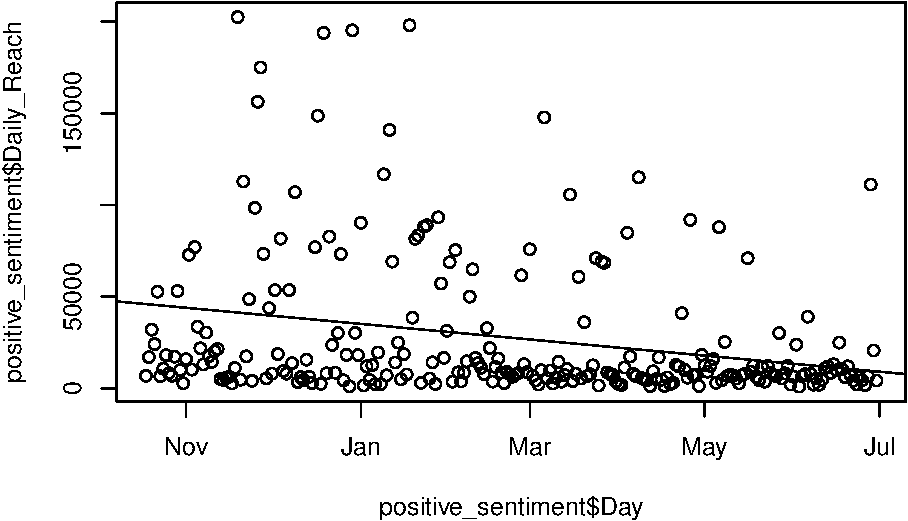
\includegraphics{_main_files/figure-latex/unnamed-chunk-14-1.pdf}

We offer two potential explanations of these results:

\begin{itemize}
\item
  \textbf{Waning Novelty}: At the beginning of the season, the new start and new possibilities often stimulate interest and positive sentiment. Over time, this novelty may fade.
\item
  \textbf{late-season Performance Decline \& Adjustment of Expectations}: fans' expectations of the team diminishes, especially given the team fails to meet those expectations in the last season, which might leads to decrease interest in online discussions about Celtics.
\end{itemize}

However, compare to our competitor, LA Lakers, for both positive and negative conversations on Twitter/X, tweets about Lakers generally decrease about 100 less reach each day compared to Celtics's. As the first explanation can be also applied to the situations faced by Lakers and other NBA franchises, team's disappointing performances might have a greater influences on fans' online engagement frequency than expected, especially given Celtics' generations' connections to the city's sport culture.

In the specific case of the Celtics, the unexpected defeat in the in-season tournament in the past two weeks, particularly when the performance of its star player was below expectations in the 1/8 Finals, could have exacerbated the decrease in online engagement in the late 2024.

\begin{verbatim}
## [1]  1  0 -1
\end{verbatim}

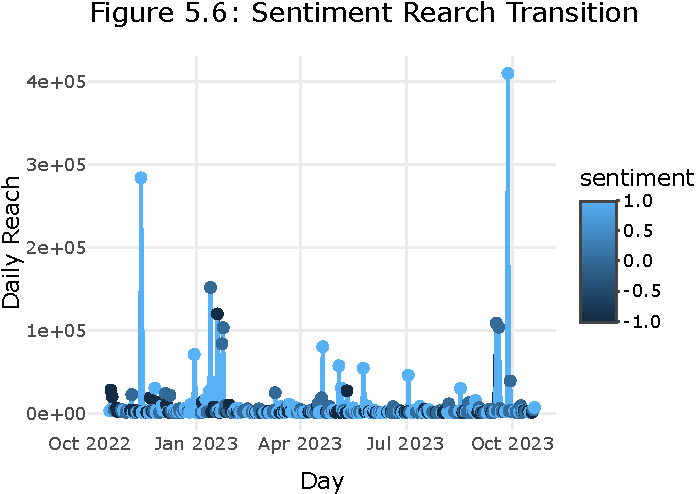
\includegraphics{_main_files/figure-latex/unnamed-chunk-15-1.pdf}

\begin{Shaded}
\begin{Highlighting}[]
\NormalTok{reg\_1la}\OtherTok{\textless{}{-}}\FunctionTok{lm}\NormalTok{(Daily\_Reach}\SpecialCharTok{\textasciitilde{}}\NormalTok{Day,positive\_sentimentla)}
\NormalTok{reg\_2la}\OtherTok{\textless{}{-}}\FunctionTok{lm}\NormalTok{(Daily\_Reach}\SpecialCharTok{\textasciitilde{}}\NormalTok{Day,negative\_sentimentla)}
\FunctionTok{stargazer}\NormalTok{(reg\_1la,reg\_2la,}\AttributeTok{type=}\StringTok{"text"}\NormalTok{,}\AttributeTok{star.cutoffs=}\FunctionTok{c}\NormalTok{(.}\DecValTok{05}\NormalTok{,.}\DecValTok{01}\NormalTok{,.}\DecValTok{001}\NormalTok{))}
\end{Highlighting}
\end{Shaded}

\begin{verbatim}
## 
## ======================================================================
##                                    Dependent variable:                
##                     --------------------------------------------------
##                                        Daily_Reach                    
##                                (1)                      (2)           
## ----------------------------------------------------------------------
## Day                        -39.990***                -32.280***       
##                              (3.659)                  (5.468)         
##                                                                       
## Constant                 784,277.100***            634,972.200***     
##                           (71,097.650)             (106,215.800)      
##                                                                       
## ----------------------------------------------------------------------
## Observations                  7,158                    2,820          
## R2                            0.016                    0.012          
## Adjusted R2                   0.016                    0.012          
## Residual Std. Error  21,511.410 (df = 7156)    20,387.020 (df = 2818) 
## F Statistic         119.431*** (df = 1; 7156) 34.856*** (df = 1; 2818)
## ======================================================================
## Note:                                    *p<0.05; **p<0.01; ***p<0.001
\end{verbatim}

\hypertarget{correlation-analysis-to-understand-reach-matrics}{%
\subsection{Correlation Analysis to Understand Reach Matrics}\label{correlation-analysis-to-understand-reach-matrics}}

To gain a deeper understanding of the metrics associated with stimulating audiences' and fans' overall reach, a correlational matrix was created. This matrix displays the correlations between reach and other observable social media metrics.

As can be directly observed in the matrix, overall:

\begin{itemize}
\item
  \textbf{Sentiment} Surprisingly, sentiments scores have almost no correlations with any other observable social media metrics.
\item
  \textbf{Overall Reach, Likes, and Replies}: Likes and replies amount are both highly positively associated with audineces' overall reach on Twitter/X.
\end{itemize}

Therefore, two specific actionable insights were determined to meet the one of the given objectives (i.e., Boost overall reach):

\begin{itemize}
\item
  \textbf{Maximize Likes to Boost Reach}: As tweets that receive more likes also get a higher daily reach. We will focus on creating content that is more likely to be liked by the audience.
\item
  \textbf{Encourage Replies for Greater Interaction}: Since replies are associated with higher daily reach, the campaign should encourage fans and franchise supporters to more actively interact and participate in conversations around the franchise.
\end{itemize}

\begin{Shaded}
\begin{Highlighting}[]
\NormalTok{melted\_cormat }\OtherTok{\textless{}{-}} \FunctionTok{melt}\NormalTok{(cor\_matrix)}
\FunctionTok{ggplot}\NormalTok{(}\AttributeTok{data =}\NormalTok{ melted\_cormat, }\FunctionTok{aes}\NormalTok{(}\AttributeTok{x=}\NormalTok{Var1, }\AttributeTok{y=}\NormalTok{Var2)) }\SpecialCharTok{+}
  \FunctionTok{geom\_tile}\NormalTok{(}\FunctionTok{aes}\NormalTok{(}\AttributeTok{fill=}\NormalTok{value), }\AttributeTok{color=}\StringTok{\textquotesingle{}white\textquotesingle{}}\NormalTok{) }\SpecialCharTok{+}
  \FunctionTok{scale\_fill\_gradient2}\NormalTok{(}\AttributeTok{low=}\StringTok{\textquotesingle{}blue\textquotesingle{}}\NormalTok{, }\AttributeTok{high=}\StringTok{\textquotesingle{}red\textquotesingle{}}\NormalTok{, }\AttributeTok{mid=}\StringTok{\textquotesingle{}grey\textquotesingle{}}\NormalTok{, }\AttributeTok{midpoint=}\DecValTok{0}\NormalTok{, }\AttributeTok{limit=}\FunctionTok{c}\NormalTok{(}\SpecialCharTok{{-}}\DecValTok{1}\NormalTok{,}\DecValTok{1}\NormalTok{), }\AttributeTok{space=}\StringTok{\textquotesingle{}Lab\textquotesingle{}}\NormalTok{, }\AttributeTok{name=}\StringTok{\textquotesingle{}Correlation\textquotesingle{}}\NormalTok{) }\SpecialCharTok{+}
  \FunctionTok{theme\_minimal}\NormalTok{() }\SpecialCharTok{+}
  \FunctionTok{theme}\NormalTok{(}\AttributeTok{axis.text.x=}\FunctionTok{element\_text}\NormalTok{(}\AttributeTok{angle=}\DecValTok{45}\NormalTok{, }\AttributeTok{vjust=}\DecValTok{1}\NormalTok{, }\AttributeTok{size=}\DecValTok{12}\NormalTok{, }\AttributeTok{hjust=}\DecValTok{1}\NormalTok{),}
        \AttributeTok{axis.text.y=}\FunctionTok{element\_text}\NormalTok{(}\AttributeTok{size=}\DecValTok{12}\NormalTok{)) }\SpecialCharTok{+}
  \FunctionTok{coord\_fixed}\NormalTok{()}
\end{Highlighting}
\end{Shaded}

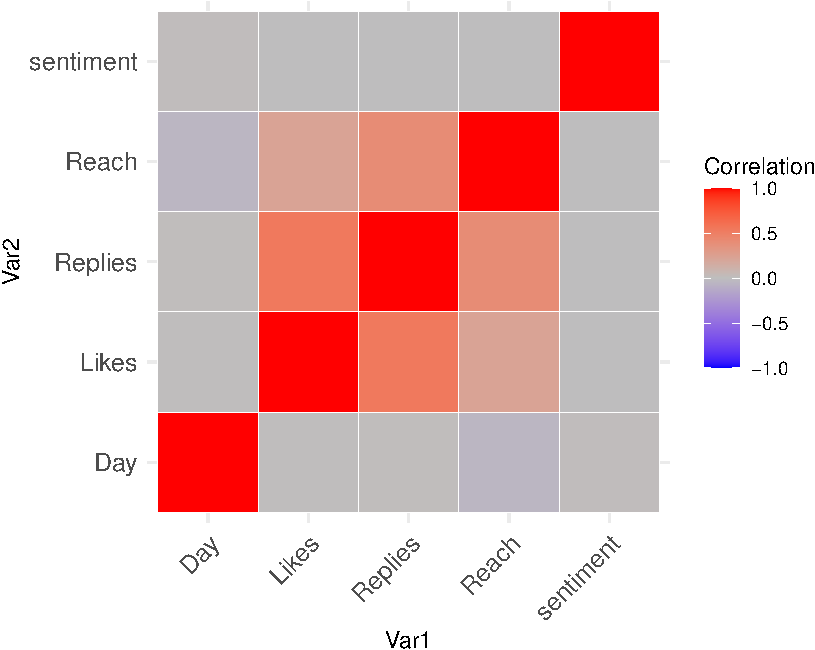
\includegraphics{_main_files/figure-latex/unnamed-chunk-18-1.pdf}

\hypertarget{distribution-of-reach-likes-replies-by-months}{%
\subsubsection{Distribution of Reach, Likes, \& Replies by Months}\label{distribution-of-reach-likes-replies-by-months}}

Given the actionable insights, box plots and density plot were utilized to understand the distributions of likes and replies by months and distribution of reach by months.

The peak in replies occurred from February to May 2023 (the regular season period after the All-Star weekend, see figure 5.7). The peak in likes was observed from May to July 2023 (from mid-NBA playoffs to the end of the NBA season, see figure 5.8), and the peak in monthly reach occurred from May to August 2023 (also covering the mid-NBA playoffs to the end of the NBA season, see figure 5.9). Given these results, the peak in replies might play a predictive role in leading to the peaks in likes and overall reach.

\begin{Shaded}
\begin{Highlighting}[]
\NormalTok{ph\_1 }\OtherTok{\textless{}{-}} \FunctionTok{ggplot}\NormalTok{(}\AttributeTok{data =}\NormalTok{ replypart, }\FunctionTok{aes}\NormalTok{(}\AttributeTok{x =}\NormalTok{ month\_factor, }\AttributeTok{y =}\NormalTok{ Reply, }\AttributeTok{fill =}\NormalTok{ month\_factor)) }\SpecialCharTok{+}
  \FunctionTok{geom\_boxplot}\NormalTok{() }\SpecialCharTok{+}
  \FunctionTok{ggtitle}\NormalTok{(}\StringTok{"Figure 5.7: Replies By Months"}\NormalTok{) }\SpecialCharTok{+}
  \FunctionTok{theme\_minimal}\NormalTok{() }\SpecialCharTok{+}
  \FunctionTok{scale\_fill\_discrete}\NormalTok{(}\AttributeTok{name =} \StringTok{"Month"}\NormalTok{) }\SpecialCharTok{+} 
  \FunctionTok{xlab}\NormalTok{(}\StringTok{"Month"}\NormalTok{) }\SpecialCharTok{+} 
  \FunctionTok{ylab}\NormalTok{(}\StringTok{"Replies"}\NormalTok{)}

\NormalTok{ph\_2 }\OtherTok{\textless{}{-}} \FunctionTok{ggplot}\NormalTok{(}\AttributeTok{data =}\NormalTok{ likepart, }\FunctionTok{aes}\NormalTok{(}\AttributeTok{x =}\NormalTok{ month\_factor, }\AttributeTok{y =}\NormalTok{ Likes, }\AttributeTok{fill =}\NormalTok{ month\_factor)) }\SpecialCharTok{+}
  \FunctionTok{geom\_boxplot}\NormalTok{() }\SpecialCharTok{+}
  \FunctionTok{ggtitle}\NormalTok{(}\StringTok{"Figure 5.8: Like By Months"}\NormalTok{) }\SpecialCharTok{+}
  \FunctionTok{theme\_minimal}\NormalTok{() }\SpecialCharTok{+}
  \FunctionTok{scale\_fill\_discrete}\NormalTok{(}\AttributeTok{name =} \StringTok{"Month"}\NormalTok{) }\SpecialCharTok{+} 
  \FunctionTok{xlab}\NormalTok{(}\StringTok{"Month"}\NormalTok{) }\SpecialCharTok{+} 
  \FunctionTok{ylab}\NormalTok{(}\StringTok{"Likes"}\NormalTok{) }\SpecialCharTok{+}
  \FunctionTok{scale\_y\_continuous}\NormalTok{(}\AttributeTok{limits =} \FunctionTok{c}\NormalTok{(}\DecValTok{0}\NormalTok{, }\DecValTok{20}\NormalTok{), }\AttributeTok{oob =}\NormalTok{ scales}\SpecialCharTok{::}\NormalTok{squish)}

\FunctionTok{grid.arrange}\NormalTok{(ph\_1, ph\_2, }\AttributeTok{ncol =} \DecValTok{2}\NormalTok{)}
\end{Highlighting}
\end{Shaded}

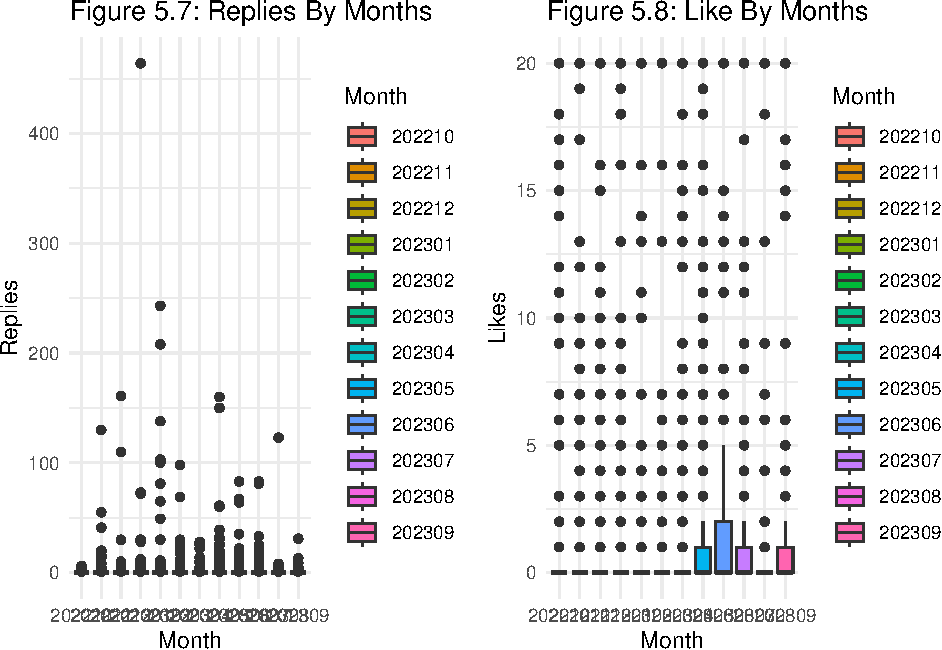
\includegraphics{_main_files/figure-latex/unnamed-chunk-20-1.pdf}

\begin{Shaded}
\begin{Highlighting}[]
\NormalTok{fan\_engage}\SpecialCharTok{$}\NormalTok{month }\OtherTok{\textless{}{-}} \FunctionTok{substr}\NormalTok{(fan\_engage}\SpecialCharTok{$}\NormalTok{Day, }\DecValTok{1}\NormalTok{, }\DecValTok{7}\NormalTok{)}

\NormalTok{Densityplot }\OtherTok{\textless{}{-}} \FunctionTok{ggplot}\NormalTok{(fan\_engage, }\FunctionTok{aes}\NormalTok{(}\AttributeTok{x =}\NormalTok{ Daily\_Reach)) }\SpecialCharTok{+}
  \FunctionTok{geom\_density}\NormalTok{(}\FunctionTok{aes}\NormalTok{(}\AttributeTok{fill =}\NormalTok{ month), }\AttributeTok{alpha =} \FloatTok{0.4}\NormalTok{) }\SpecialCharTok{+}
  \FunctionTok{geom\_vline}\NormalTok{(}\FunctionTok{aes}\NormalTok{(}\AttributeTok{xintercept =} \FunctionTok{mean}\NormalTok{(Daily\_Reach)), }\AttributeTok{linetype =} \StringTok{"dashed"}\NormalTok{, }\AttributeTok{color =} \StringTok{"red"}\NormalTok{) }\SpecialCharTok{+}
  \FunctionTok{ggtitle}\NormalTok{(}\StringTok{"Figure 5.9: Density Plot for Reach Distribution by Month"}\NormalTok{) }\SpecialCharTok{+}
  \FunctionTok{xlab}\NormalTok{(}\StringTok{"Reach Number"}\NormalTok{) }\SpecialCharTok{+}
  \FunctionTok{ylab}\NormalTok{(}\StringTok{"Density"}\NormalTok{) }\SpecialCharTok{+}
  \FunctionTok{theme\_minimal}\NormalTok{()}
\FunctionTok{print}\NormalTok{(Densityplot)}
\end{Highlighting}
\end{Shaded}

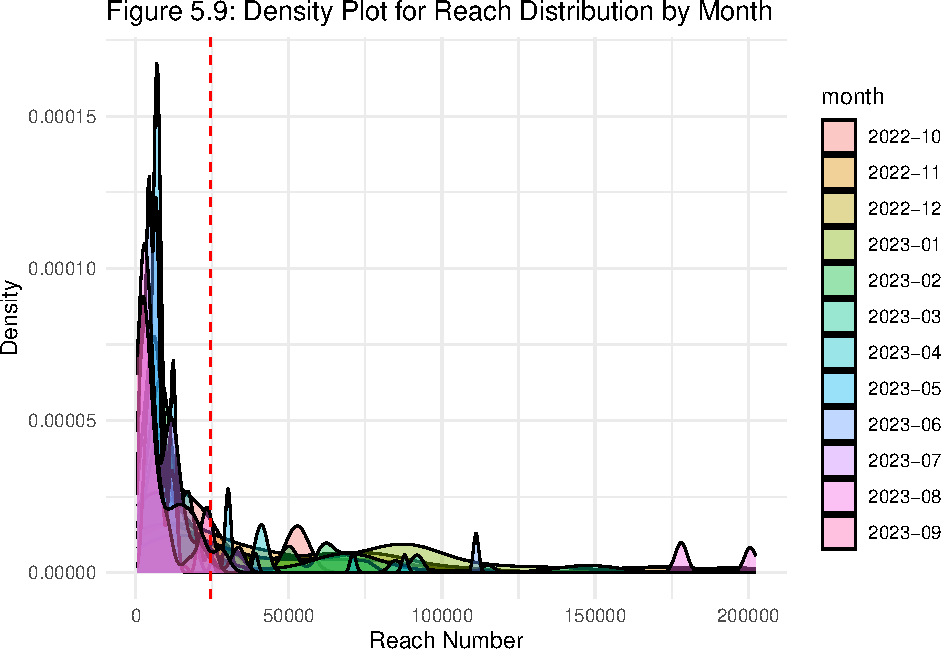
\includegraphics{_main_files/figure-latex/unnamed-chunk-20-2.pdf}

\hypertarget{a-2024-customized-pre-playoff-twitterx-campaign}{%
\subsection{A 2024 Customized Pre-Playoff Twitter/X Campaign}\label{a-2024-customized-pre-playoff-twitterx-campaign}}

Given the above insights, we aim to launch a customized campaign on Twitter/X. This campaign intends to capitalize on the increased engagement before the 2024 playoffs to build momentum through running a series of interactive Twitter/X campaigns that encouraging replies.

Given the peak time range of reply metrics in the last season, which mainly occurred at the remaining regular season period since the All-Star weekend, this campaign will start from the week after All-Star and end before the 2024 NBA playoffs.

\hypertarget{campaign-strategies}{%
\chapter{Campaign Strategies}\label{campaign-strategies}}

\hypertarget{a-customized-campaign-to-enahnce-engagement-on-tiktok-1}{%
\section{A Customized Campaign to Enahnce Engagement on TikTok}\label{a-customized-campaign-to-enahnce-engagement-on-tiktok-1}}

\hypertarget{content-strategy-for-tiktok}{%
\subsection{Content Strategy For TikTok}\label{content-strategy-for-tiktok}}

Based on the hashtags and words frequently mentioned in TikTok conversations about the Celtics, as collected from Meltwater, it is evident that a substantial portion of these discussions centers around fan identity and support. This is exemplified by the popularity of fan slogans such as ``\#bleedgreen'', ``\#celticswin'', and ``\#celticsnation'' (see figure 6.1).

\begin{figure}
\centering
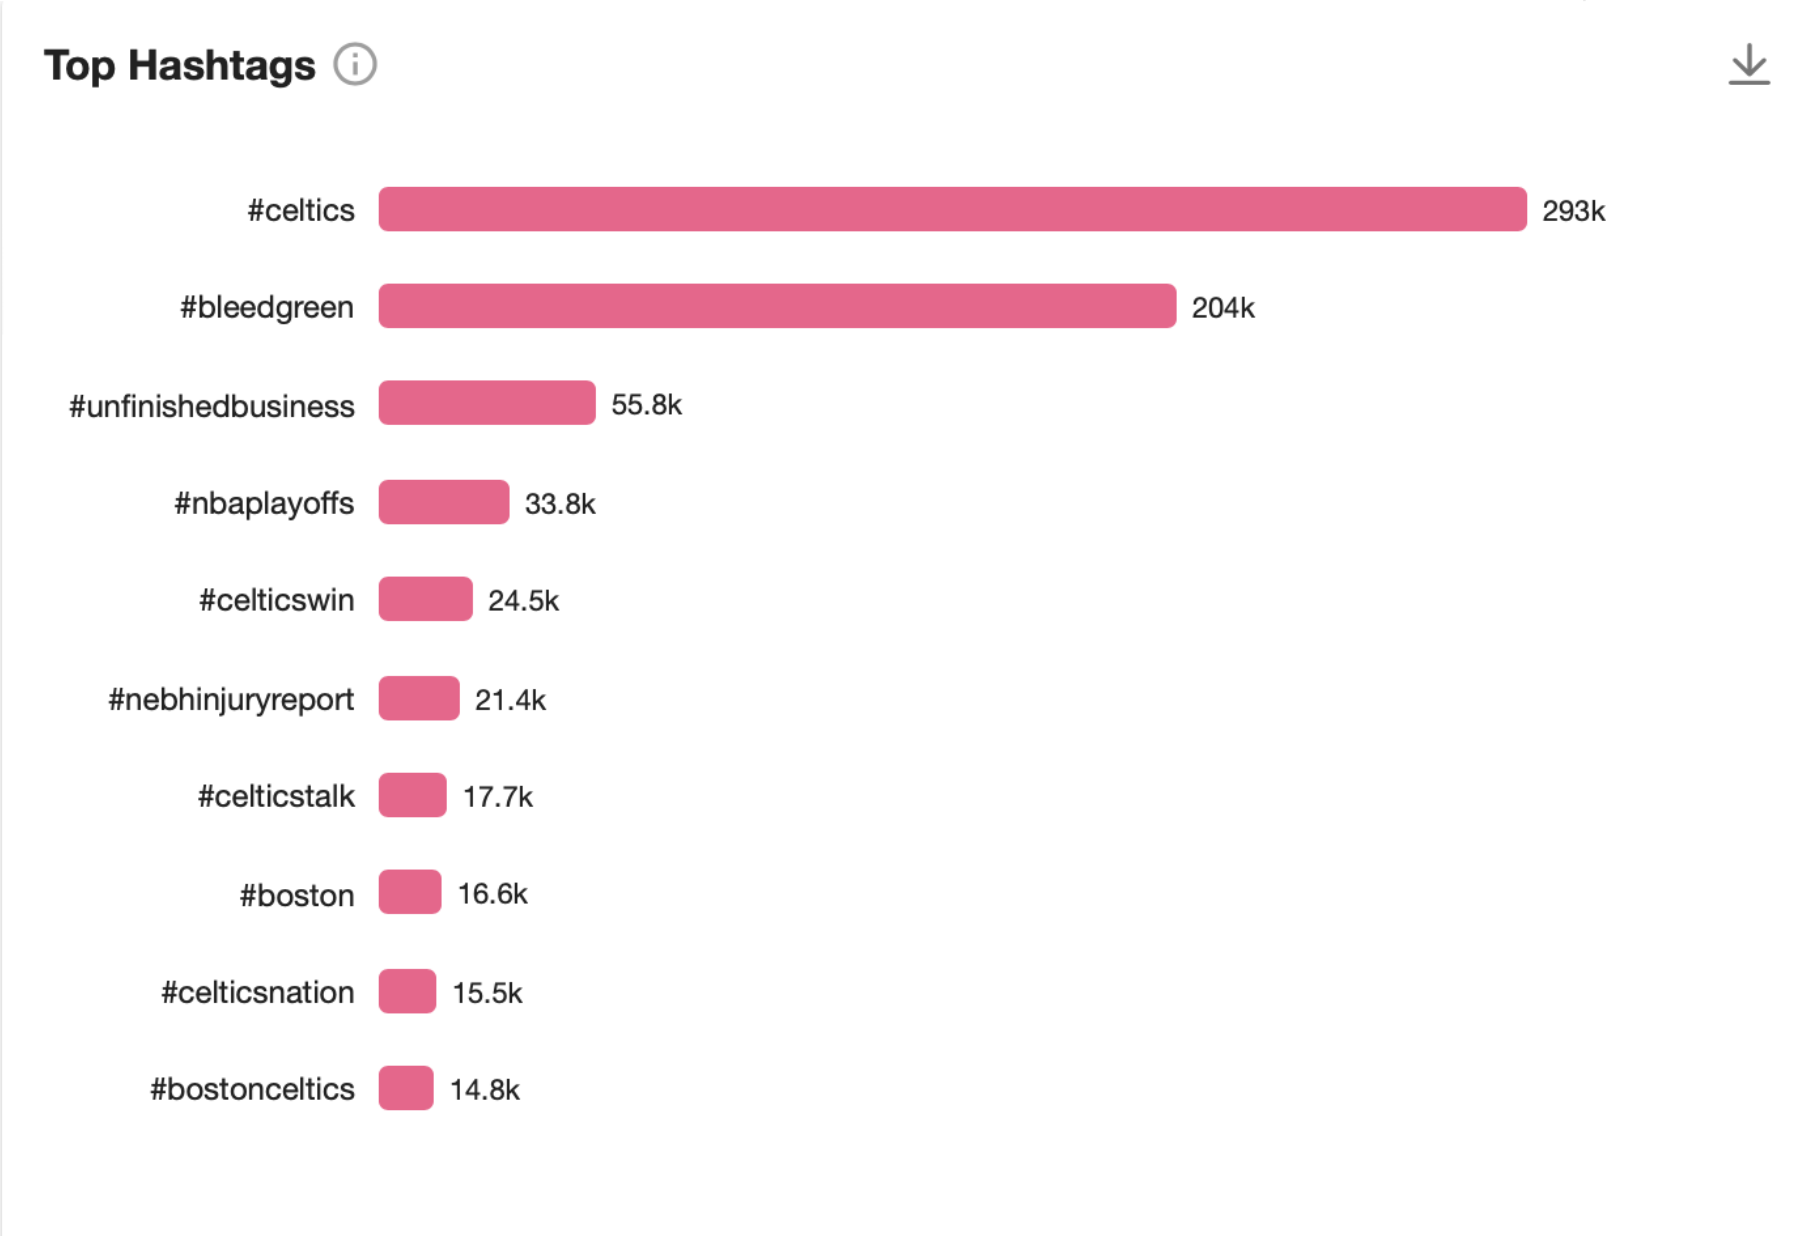
\includegraphics{4.png}
\caption{Top Hashtags}
\end{figure}

Additionally, among these conversations mentioning the Celtics, the recurrent mention of elements like ``person'', ``tank top'', ``footwear'', ``cap hat'', and ``stadium'' is likely indicative of references to players, potentially focusing on their sportswear during regular training scenes (see figure 6.2).

\begin{figure}
\centering
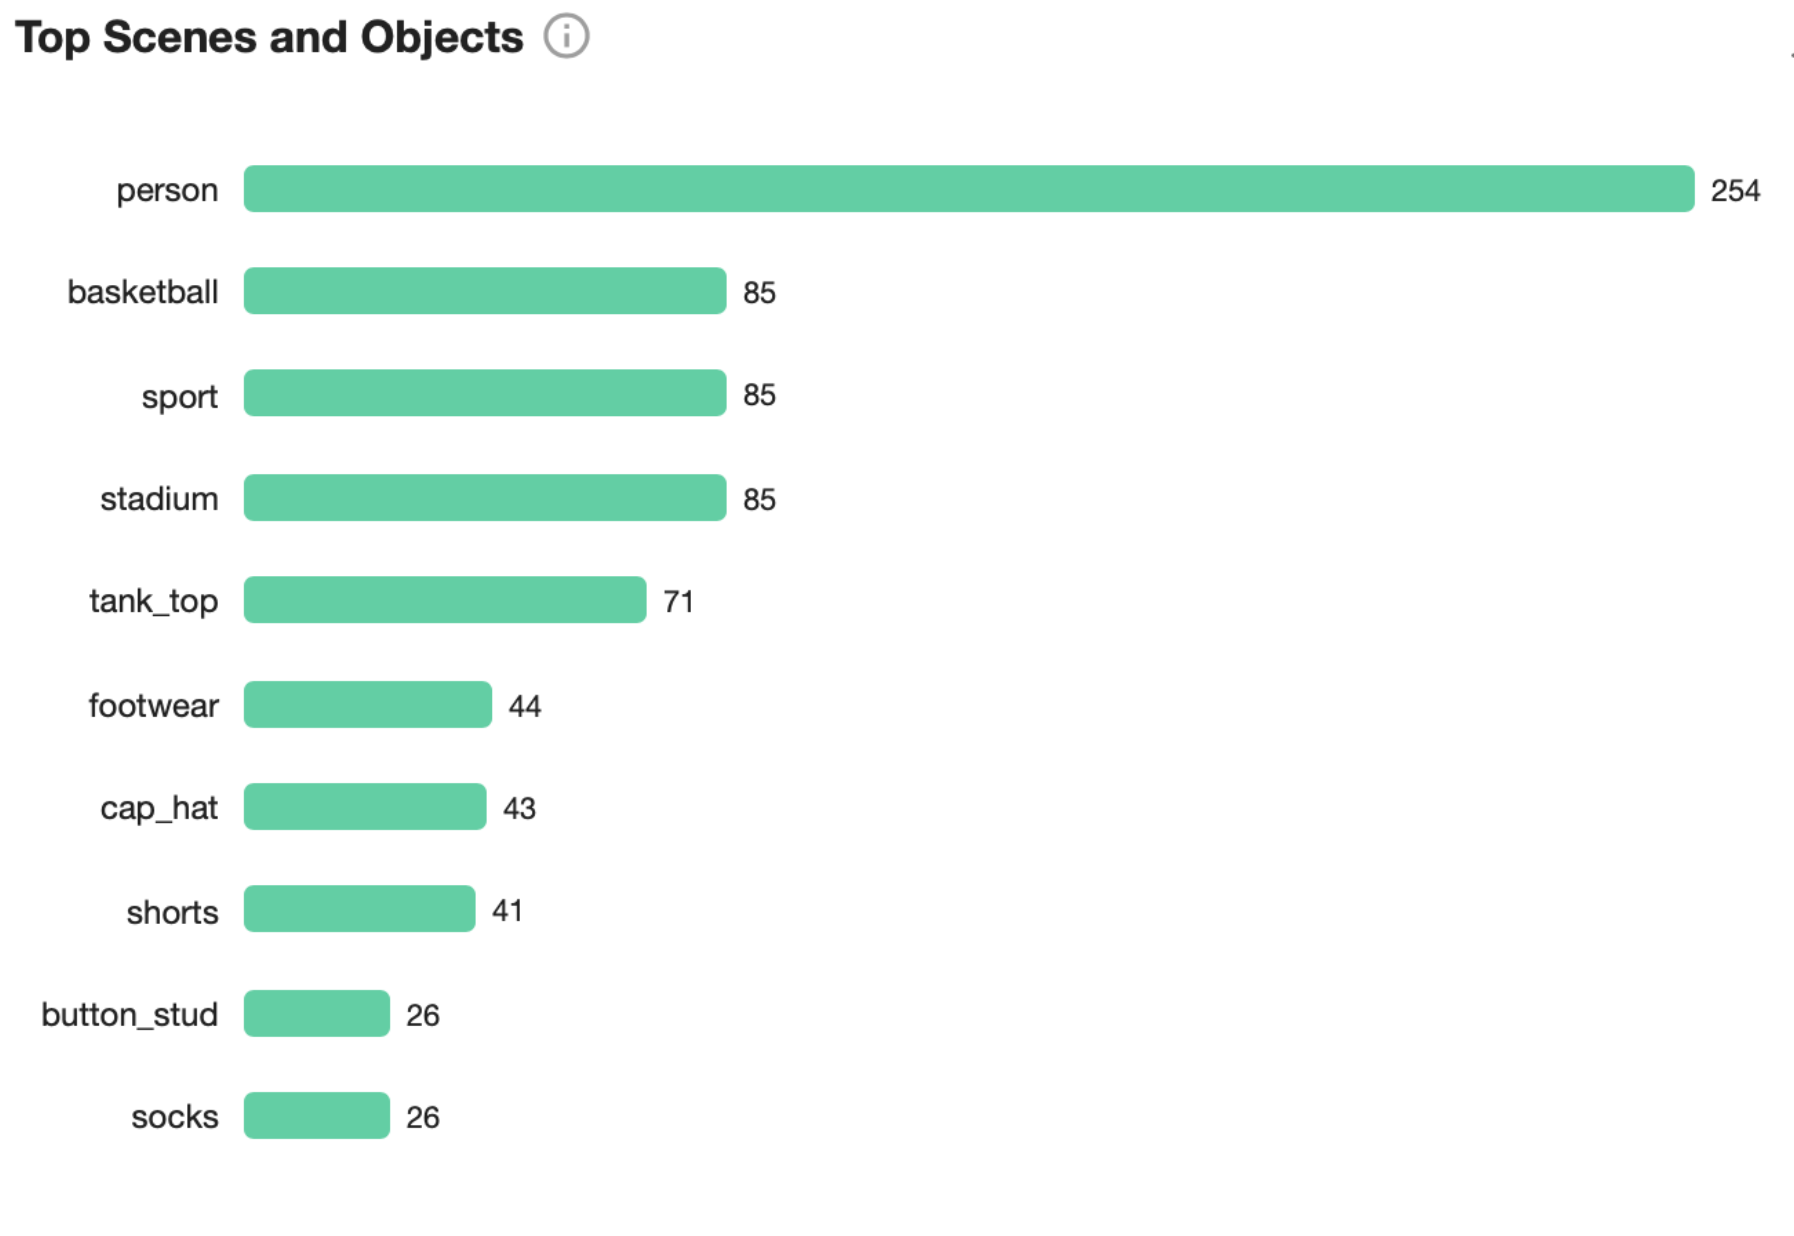
\includegraphics{5.png}
\caption{Top Mentioned Words}
\end{figure}

\hypertarget{a-customized-bleedgreen-campaign-on-tiktok}{%
\subsection{A Customized \#BleedGreen Campaign on TikTok}\label{a-customized-bleedgreen-campaign-on-tiktok}}

Named the ``\#BleedGreen'' campaign, this TikTok-centered initiative aims to appeal to Celtics fans to purchase and wear sportswear modeled after popular players (e.g., sneakers) or Celtics-related apparel, and share these moments on TikTok to proudly signify their Celtics fan identity.

To be specific:

\begin{enumerate}
\def\labelenumi{\arabic{enumi})}
\item
  By partnering with popular TikTok influencers and brands in the realms of sport fashion and basketball culture, we aim to leverage TikTok's unique media experience (e.g., click to view product information in videos) to create various content. This includes collaborating with influencers to produce a series of review videos introducing the daily wear of Jayson Tatum and Jaylen Brown, and partnering with popular sports brands to stream events where fans can participate in designing the new season's official jersey. During these events, fans will be encouraged to rank Celtics's classical jersey and other fans' designs. And we will award the winner of the design games the tickets to watch a live game in Celtics courtside VIP area.
\item
  Additionally, with a focus on creating content that has the potential to go viral on TikTok, we will encourage Celtics fans to ``show their fan identity'' on the platform by sharing their Celtics-related apparel. In our appeals, we will initially collaborate with Hall of Fame Celtics players to make a series of videos of them wearing fan-design jersey, and publish these videos on TikTok using popular hashtags such as \#celticsnation and \#bleedgreen in their videos. And then we will encourage our useres to also use these hashtags in the videos they wearing Celtics-related apparel. This strategy aims to ensure that these contents reach a larger fan community on TikTok who are interested in the sportswear culture surrounding the Celtics, as shown in our analysis.
\end{enumerate}

\hypertarget{a-pre-playoff-campaign-on-twitterx}{%
\section{A Pre-playoff Campaign on Twitter/X}\label{a-pre-playoff-campaign-on-twitterx}}

\hypertarget{topic-network-analysis}{%
\subsection{Topic Network Analysis}\label{topic-network-analysis}}

As we aim to promote audiences' overall engagements in fan-engagement conversations around the franchise, for the Twitter/X campaign, the ``sna'' package in r was utilized to perform a topic network analysis to see what other conversations can predict the popularity of fan engagement topics.

Given that our sample data spans a one-year time range, we divided this duration into two-month segments, each defined as a unique time period. Figure 6.3 illustrates the dynamic relationship between topics across these time periods. It shows how the popularity of topic A in one period can influence or predict the popularity of topic B in the subsequent period. The figure also includes edge weights, representing the transition frequency values between two topics. These weights provide insights into how strongly one topic is likely to lead to increased engagement in another, enabling us to strategically focus our efforts on key topics that drive fan engagement.

Interpreting from figure 6.3:

\begin{itemize}
\item
  \textbf{Fan engagement topic as predictor}: Popularity about fan community (topic 7) in a previous period predicts the popularity of conversations around winning appeals (topic 5) in a following period, which in turn predicts the popularity of discussions around Celtics slogan (topic 4) in a subsequent period.
\item
  \textbf{Topic 6 and 4}: Popularity of conversations around game strategies (topic 6) predicts the popularity of conversations around Celtics slogan (topic 4) in the following period.
\item
  \textbf{Topic 8 and 7}: Popularity of conversations around team-management (topic 8) predicts the popularity of conversations around fan community (topic 7) in the following period.
\end{itemize}

\begin{Shaded}
\begin{Highlighting}[]
\NormalTok{transition\_freq }\OtherTok{\textless{}{-}}\NormalTok{ transitions }\SpecialCharTok{\%\textgreater{}\%}
  \FunctionTok{group\_by}\NormalTok{(Transition) }\SpecialCharTok{\%\textgreater{}\%}
  \FunctionTok{summarise}\NormalTok{(}\AttributeTok{Frequency =} \FunctionTok{n}\NormalTok{())}

\NormalTok{edges }\OtherTok{\textless{}{-}} \FunctionTok{strsplit}\NormalTok{(}\FunctionTok{as.character}\NormalTok{(transition\_freq}\SpecialCharTok{$}\NormalTok{Transition), }\StringTok{"{-}\textgreater{}"}\NormalTok{) }\SpecialCharTok{\%\textgreater{}\%}
  \FunctionTok{lapply}\NormalTok{(}\ControlFlowTok{function}\NormalTok{(x) }\ControlFlowTok{if}\NormalTok{ (}\SpecialCharTok{!}\FunctionTok{any}\NormalTok{(}\FunctionTok{is.na}\NormalTok{(x))) }\FunctionTok{cbind}\NormalTok{(x[}\DecValTok{1}\NormalTok{], x[}\DecValTok{2}\NormalTok{])) }\SpecialCharTok{\%\textgreater{}\%}
  \FunctionTok{do.call}\NormalTok{(rbind, .) }\SpecialCharTok{\%\textgreater{}\%}
  \FunctionTok{na.omit}\NormalTok{() }\SpecialCharTok{\%\textgreater{}\%} 
  \FunctionTok{as.matrix}\NormalTok{()}

\NormalTok{filtered\_edges }\OtherTok{\textless{}{-}}\NormalTok{ edges[transition\_freq}\SpecialCharTok{$}\NormalTok{Frequency }\SpecialCharTok{\textgreater{}=} \DecValTok{5}\NormalTok{, ]}
\NormalTok{network }\OtherTok{\textless{}{-}} \FunctionTok{graph\_from\_edgelist}\NormalTok{(filtered\_edges, }\AttributeTok{directed =} \ConstantTok{TRUE}\NormalTok{)}
\FunctionTok{E}\NormalTok{(network)}\SpecialCharTok{$}\NormalTok{weight }\OtherTok{\textless{}{-}}\NormalTok{ transition\_freq}\SpecialCharTok{$}\NormalTok{Frequency[transition\_freq}\SpecialCharTok{$}\NormalTok{Frequency }\SpecialCharTok{\textgreater{}=} \DecValTok{5}\NormalTok{]}
\end{Highlighting}
\end{Shaded}

\begin{figure}
\centering
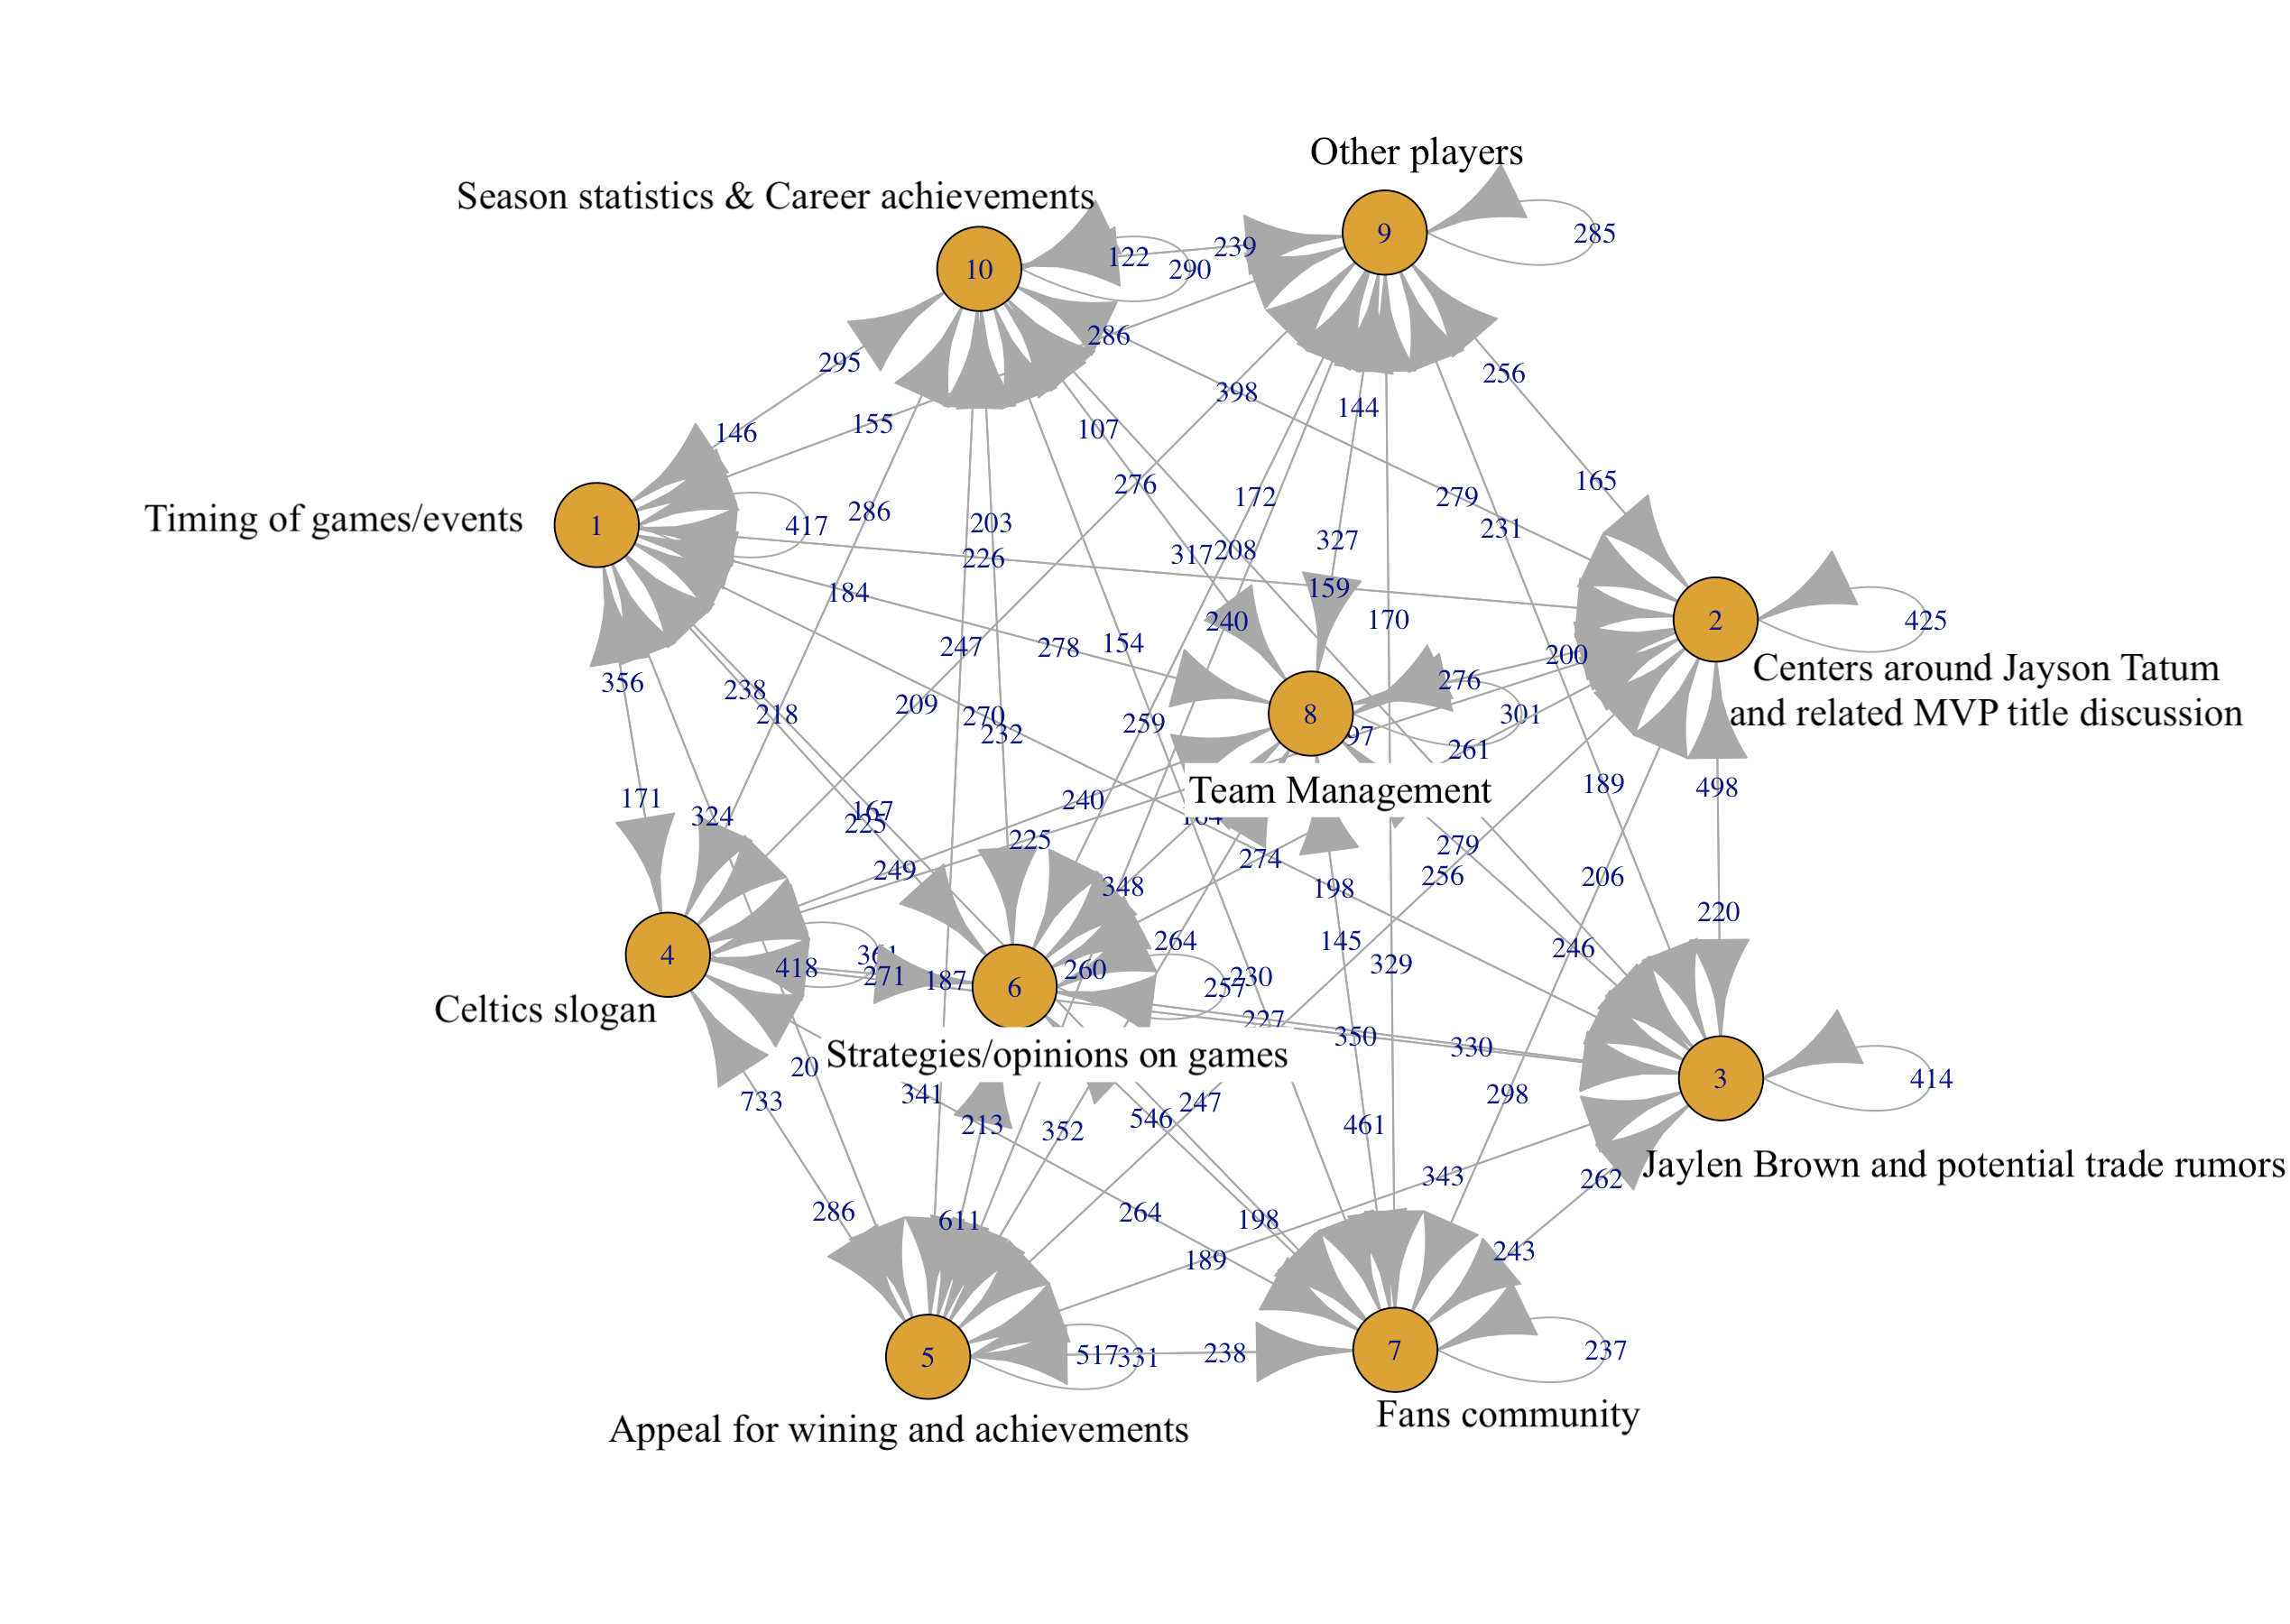
\includegraphics{8.jpg}
\caption{Topic Network Prediction Model}
\end{figure}

\hypertarget{customized-strategies-for-pre-playoff}{%
\subsection{Customized Strategies for Pre-playoff}\label{customized-strategies-for-pre-playoff}}

\begin{itemize}
\item
  \textbf{Celtics Fan Stories (Customized for Topic 7)}: Aiming to let our fans to feel valued and see their personal experience as an integral part of the franchise's and community's shared experiences, we will select and feature fan stories on Celtics' official Twitter/X feed and the jumbotron during games. This also aims to emphasize the collective identity and unity of the fan community.
\item
  \textbf{Weekly Roundtable (Customized for Topic 8)}: We will host a series of weekly roundtable discussion with a panel of players, coaches, analysts to discuss team's weekly performance and answer fans' most interested questions. By doing this, we aim to let the Celtics' fans feel like they are part of the team's inner circle, which might help to strengthen trust and reciprocal relationships among fan community.
\item
  \textbf{Be the Coach (Customized for Topic 6)}: Aiming to increase fan's emotional and timely investment in the franchise's success and deepen their loyalty, we will engage them with weekly strategic/controversial questions on Twitter/X invites them to participate actively in the discourses related to game strategies, player performances, or hypothetical matchups. Through using specific hashtags and collaborate with social monitoring platforms to track the ongoing of these conversations, we aim to use dynamic data to further simulate the active creations of various sub-communities within the larger Celtics fan base, fostering niche groups that bond over specific topics or events around Celtics culture.
\end{itemize}

  \bibliography{book.bib,packages.bib}

\end{document}
